\documentclass[preprint,12pt,authoryear]{elsarticle}
\usepackage{amsmath,amsfonts}
\usepackage{algorithmic}
\usepackage{algorithm}
\usepackage{array}
\usepackage{booktabs}
\usepackage{multirow}
\usepackage{textcomp}
\usepackage{url}
\usepackage{graphicx}
\usepackage{tikz}
\usepackage{enumitem}
\usepackage{lineno}
\usepackage{placeins}
\usepackage{longtable}
\usepackage{listings}
\lstset{basicstyle=\ttfamily\scriptsize,breaklines=true,columns=fullflexible,keepspaces=true,frame=single,framerule=0.3pt,xleftmargin=0pt,aboveskip=4pt,belowskip=4pt,breakatwhitespace=true}
\usepackage[export]{adjustbox}
\usetikzlibrary{fit,backgrounds,calc}
\usepackage{pgfplots}
\usepgfplotslibrary{groupplots}
\pgfplotsset{compat=1.16}
\newcommand{\sysZS}{\textsc{Zero-Shot}}
\newcommand{\sysRO}{\textsc{Retrieval-Only}}
\newcommand{\sysMA}{\textsc{Multi-Agent}}
\newcommand{\sysNC}{\textsc{Cadence-NC}}
\newcommand{\sysFull}{\textsc{Cadence-Full}}
\newcommand{\modl}[1]{{\tiny\ttfamily #1}}
\setlength{\emergencystretch}{3em}
\renewcommand{\_}{\textunderscore\allowbreak{}}
\usetikzlibrary{arrows.meta, positioning, shapes.geometric}
\journal{Information and Software Technology}
\modulolinenumbers[5]

\begin{document}

\begin{frontmatter}

\title{CADENCE: Case-Grounded, Deliberation-Driven, and Solver-Verified Architectural Decision-Making with Large Language Models}

\author{Quang-Vinh Dang}
\ead{vinh.dq4@buv.edu.vn}
\address{British University Vietnam, Hung Yen, Vietnam}

\begin{abstract}
\textbf{Context:} Large language models (LLMs) are increasingly used to draft architecture decision records (ADRs). Existing approaches generate decisions from a prompt, retrieved precedents, or role-based agents, but none checks whether the resulting decision actually addresses the quality attributes at stake within what a team can build. Architecture optimization offers such checks, but only on design spaces that experts have specified by hand.
\textbf{Objective:} We aim to join the two lines of work, and to find out which parts of an LLM decision pipeline improve the decision and where such a pipeline fails.
\textbf{Method:} We present CADENCE, which retrieves precedent ADRs from a corpus of 6{,}173 mined records, lets five agents each advocate one ISO/IEC~25010 quality attribute while grounded in a tactic knowledge graph, encodes the decision's tactic commitments as a lexicographic weighted MaxSAT problem in the Z3 solver with an LLM repair loop, and scores the result. We evaluate it on 30 held-out ADRs from open-source projects in a paired ablation that adds one stage at a time, using a local 1.5B-parameter backbone, two tactic budgets, Wilcoxon tests with Holm correction, a length-controlled analysis, and a comparison with published frontier-model generations.
\textbf{Results:} Retrieval slightly improves agreement with the recorded decisions. Multi-agent deliberation lowers it on all four metrics, by more than its shorter output explains. The solver correctly flags 29 of 30 deliberated decisions as leaving required quality attributes without a committed tactic. Repair raises mean coverage from 0.57 to 1.63 of five attributes but makes only one decision feasible. Extra budget does not help, because the committed tactics cluster on too few attributes. The critique stage does not change the decision text; its residual weaknesses, rendered as consequences, significantly increase agreement. The paired design also shows that an earlier small-sample gain attributed to critique was sampling noise.
\textbf{Conclusion:} Formal verification is a reliable detector of quality-attribute gaps in LLM-drafted decisions, but repairing the text after the fact is not enough. Decisions should commit to tactics in a structured form, and LLM decision support should be evaluated by more than agreement with a single recorded ADR.
\end{abstract}

\begin{keyword}
Software architecture \sep architectural decision-making \sep architecture decision records \sep architectural tactics \sep large language models \sep constraint solving \sep empirical evaluation
\end{keyword}

\end{frontmatter}

\linenumbers

\section{Introduction}

Architectural decisions are the design choices that are expensive to reverse: introducing a message queue, splitting a service, adopting event sourcing, choosing where encryption terminates. Software architecture research has treated these decisions, and the rationale behind them, as first-class architectural knowledge for two decades~\citep{jansen2005,kruchten2004,tang2006}, and practitioners record them as architecture decision records (ADRs)~\citep{tyree2005}, a practice now visible in hundreds of open-source repositories~\citep{buchgeher2023adr}. Empirical studies of how architects actually decide report a consistent picture. Decisions are made under time pressure with partial knowledge of precedent~\citep{vanvliet2016,weinreich2015}; trade-offs among quality attributes are weighed informally and often implicitly~\citep{zalewski2017,falessi2011}; and the process is exposed to cognitive biases such as anchoring on the first option considered~\citep{borowa2021,razavian2016}. Systematic methods exist to counter this --- ATAM and CBAM for trade-off analysis~\citep{kazman1998atam,kazman2001cbam}, tactic catalogs linking design choices to quality attributes~\citep{bachmann2003,bass2021saip}, and search-based architecture optimization~\citep{aleti2013,koziolek2011peropteryx} --- but they demand expert effort or a formal architecture model that is rarely available when a decision is first drafted.

Large language models (LLMs) lower that effort, and the software architecture community has started to use them for exactly this task: drafting ADRs from a decision context~\citep{dhar2024llm}, grounding the draft in mined precedent~\citep{contextmatters2026}, splitting architecture design across role-based agents~\citep{zhang2025maad}, and supporting quality-attribute or ATAM-style reasoning~\citep{diazpace2025,capilla2025atam}. Recent surveys and roadmaps record the same open problem across this work~\citep{hou2024,esposito2026,schmid2025}: an LLM's decision is text, and nothing in these pipelines checks that the tactics it commits to actually cover the quality attributes at stake, or that they fit within what the team can build. In MAAD, for instance, the final evaluation step is another LLM call~\citep{zhang2025maad}. Conversely, the architecture-optimization tradition offers exactly that kind of check, but expects its design space to be specified by hand~\citep{aleti2013,martens2010}. The two lines have not been joined.

This paper joins them. We present CADENCE, an approach to LLM-assisted architectural decision-making that treats the LLM as a generator of decision alternatives and rationale, and treats the decision's tactic commitments as a design-space problem to be checked formally. CADENCE has four stages. (1)~It retrieves the closest precedent ADRs from a corpus of 6{,}173 mined records~\citep{buchgeher2023adr}. (2)~Five agents, each advocating one ISO/IEC~25010-derived quality attribute~\citep{iso25010} and grounded in a 26-tactic knowledge graph with explicit trade-off edges, deliberate over a candidate decision, so that competing concerns are argued for rather than averaged away. (3)~The tactics the candidate commits to are encoded as a lexicographic weighted MaxSAT problem in the Z3 SMT solver: cover every required quality attribute within a tactic budget $B$, then minimize trade-off cost. If the encoding is unsatisfiable, the uncovered attributes drive an LLM repair loop. (4)~A finalization pass combines a deterministic utility score, computed from the solver's selection and the graph's trade-off edges, with an LLM critique of residual weaknesses.

We evaluate CADENCE as one would evaluate a decision-support tool for software architects, on held-out human-authored ADRs and with an ablation in which each system adds one stage to the previous one. The evaluation addresses four research questions:
\begin{description}[leftmargin=1.2em,style=nextline]
\item[RQ1 (stage contribution)] How does each stage --- precedent retrieval, quality-attribute deliberation, solver verification, and critique --- change agreement with the decisions architects actually recorded?
\item[RQ2 (feasibility)] Can solver verification with repair make an LLM-proposed decision cover all required quality attributes within a tactic budget, and how often does it succeed as the budget gains slack?
\item[RQ3 (external reference)] How do CADENCE's decisions compare with ADRs generated by frontier LLMs on the same items, as published in an independent replication package~\citep{contextmatters-zenodo}?
\item[RQ4 (measurement)] How well do reference-based text metrics, the standard instrument in LLM-for-ADR studies, capture differences between structured, multi-stage decision output and free-form generations?
\end{description}

The paper makes four contributions to software architecture research.
\begin{enumerate}[leftmargin=*]
\item \emph{An approach that couples LLM-generated decision alternatives with formal design-space verification.} CADENCE links the LLM-for-ADR line of work to tactic-based reasoning~\citep{bachmann2003,bass2021saip} and to solver-based architecture optimization~\citep{aleti2013}. To our knowledge it is the first ADR-generation approach in which a decision's quality-attribute coverage is checked by a solver rather than judged by another LLM (Table~\ref{tab:relatedwork}).
\item \emph{An encoding from free-text deliberation to a budgeted coverage problem.} We show that the encoding must be lexicographic: under a weighted sum, a large trade-off weight can outvote coverage, and a decision that leaves an attribute uncovered is then reported as optimal (Section~\ref{sec:method-stage3}).
\item \emph{A paired ablation study on held-out ADRs from open-source projects.} From the deliberation onward, all systems share the same intermediate outputs, so each comparison isolates exactly one stage. The study shows that the solver reliably detects decisions that leave quality attributes uncovered (29 of 30 items), and that the binding constraint is the diversity of the tactics a decision commits to, not the tactic budget. We release the per-item outputs and solver diagnostics.
\item \emph{Two lessons about measurement.} First, reference-based metrics penalize CADENCE's output beyond what its shorter length explains. Second, ablations of stochastic pipelines that re-sample shared stages can produce spurious stage effects. Our own earlier small-sample result for the critique stage was one such effect. Both lessons bear on how LLM-for-architecture studies should report results~\citep{evtikhiev2023,roy2021}.
\end{enumerate}

Section~\ref{sec:related} positions CADENCE in the architecture-knowledge, decision-making, optimization and LLM-for-architecture literature. Section~\ref{sec:method} presents the approach. Section~\ref{sec:evaluation} reports the evaluation by research question, Section~\ref{sec:discussion} discusses implications for practice and research and the threats to validity, and Section~\ref{sec:conclusion} concludes.

\section{Related Work}
\label{sec:related}

CADENCE draws on six bodies of software engineering research: the view of architecture as a set of design decisions and the management of the knowledge behind them; empirical work on how architects decide; trade-off analysis and quantitative selection methods; automated architecture optimization; architectural tactics and their quality-attribute relationships; and the recent use of large language models in software architecture. We review each and close the section with a summary of how CADENCE differs from the closest prior work (Table~\ref{tab:relatedwork}).

\subsection{Architectural decisions and architecture knowledge}

\citet{jansen2005} argued that a software architecture is best understood as a set of architectural design decisions, and that losing those decisions and their rationale, rather than losing the structure itself, is what makes architectures hard to evolve. \citet{tyree2005} gave the decision record its practical form, with fields for the issue, assumptions, alternatives, argument and implications that today's ADR templates still carry, and \citet{kruchten2004} classified decisions (existence, property and executive decisions) and the relations between them, such as constrains, forbids and conflicts with. \citet{zimmermann2009} made such relations operational: their reusable decision models carry dependency relations and formal integrity constraints, so that a tool can check whether a set of decisions is consistent. CADENCE inherits this idea of constraint-checked decisions. Its constraints are narrower (a tactic budget and quality-attribute coverage), but they are checked by a solver against an explicit tactic model rather than by rules over a decision tree, and the decisions themselves are proposed by language-model agents.

The architecture knowledge management (AKM) literature documents why this matters in practice. Practitioners value design rationale but seldom record it~\citep{tang2006}; AKM tools support capture, sharing and reasoning to different degrees~\citep{tang2010}; and a ten-year retrospective names the cost of capture and the weak reuse of captured knowledge as the main obstacles to adoption~\citep{capilla2016}. Open-source projects now publish ADRs in large numbers, although adoption per repository remains sparse~\citep{buchgeher2023adr}. CADENCE treats these mined ADRs as reusable knowledge: Stage~1 retrieves them as precedents for a new decision, and Stages~2--4 record the rationale (agent positions, solver verdict, repair history, critique) as a by-product of making the decision.

\subsection{Architectural decision-making in practice}

Architects rarely optimize. They satisfice under bounded rationality, decide in groups, and are subject to cognitive biases~\citep{vanvliet2016}. Anchoring and confirmation bias have been observed in architecture decisions~\citep{zalewski2017} and linked to architectural technical debt~\citep{borowa2021}, while prompting designers to reflect on their reasoning improves design decisions~\citep{razavian2016}. An expert survey reports which kinds of decisions and which influence factors, including cost and team expertise, dominate in practice~\citep{weinreich2015}. A comparative survey of decision-making techniques for architecture design describes the assumptions behind weighted scoring, AHP and related multi-criteria methods~\citep{falessi2011}. These findings shape three design choices in CADENCE. The adversarial quality-attribute advocates are a structured form of group deliberation intended to keep any single viewpoint from dominating; the separate critique pass is a form of reflection; and the lexicographic objective in Stage~3 is a deliberate choice among the multi-criteria techniques that \citet{falessi2011} compare, made so that coverage of a required attribute can never be traded away for a lower trade-off cost (Section~\ref{sec:method-stage3}).

\subsection{Trade-off analysis and quantitative selection}

The Architecture Tradeoff Analysis Method (ATAM) organizes an evaluation around a quality-attribute utility tree and identifies sensitivity points and trade-off points in a candidate architecture~\citep{kazman1998atam}. The Cost Benefit Analysis Method (CBAM) extends it by choosing among architectural strategies according to their benefit per unit cost under a budget~\citep{kazman2001cbam}; experience with CBAM showed that eliciting reliable utilities from stakeholders is the hardest step~\citep{moore2003}. \citet{alnaeem2005} combined multi-criteria scoring with integer programming to select design alternatives under quality and resource constraints. CADENCE's Stage~3 belongs to this tradition: it, too, selects architectural strategies under a budget so as to satisfy quality-attribute requirements. What differs is where the inputs come from. CBAM and \citet{alnaeem2005} assume that stakeholders enumerate the alternatives and supply the scores; CADENCE derives candidate tactics from a natural-language decision context through retrieval and deliberation, scores trade-offs from an explicit tactic model, and repairs a candidate automatically when the selection is infeasible. It is meant to support such methods, not to replace a stakeholder-driven evaluation.

\subsection{Automated architecture optimization}

A systematic review of software architecture optimization classifies approaches by problem, degrees of freedom, quality evaluation and optimization strategy, and finds that most rely on quantitative quality models and metaheuristic search~\citep{aleti2013}. Representative tools search over component and deployment models for performance, reliability and cost~\citep{martens2010,aleti2009archeopterix}; PerOpteryx applies architectural tactics as search operators in multi-objective optimization~\citep{koziolek2011peropteryx}; and recent work explores many-objective refactoring of software models~\citep{cortellessa2023}. Solver-based synthesis of architectures from formal style specifications~\citep{bagheri2016} and the SAT/CSP/SMT analysis of feature models, including optimal configuration under cost constraints~\citep{benavides2010}, show that constraint solvers are well established for architecture-level choices. In the terms of \citet{aleti2013}, CADENCE's degree of freedom is the selection of tactics, its quality evaluation is a qualitative tactic model plus an LLM critique, and its strategy is exact (weighted MaxSAT/SMT) rather than metaheuristic. It does not need a component model or performance predictions, which makes it applicable earlier than model-based optimizers, but its quality evaluation is correspondingly coarser. PerOpteryx in particular already automates tactic application across several quality attributes; CADENCE differs in starting from natural-language context and precedents instead of an architecture model, and in using a solver to verify and repair an LLM-proposed decision rather than to search a model-defined design space.

\subsection{Architectural tactics and quality attributes}

Tactics were introduced as design primitives derived from quality-attribute reasoning frameworks~\citep{bachmann2003} and are catalogued in \citet{bass2021saip}. Tactics interact with architecture patterns and with one another, sometimes with negative effects on other attributes~\citep{harrison2010,harrison2007}; such relationships have been mined from developer discussions~\citep{bi2021}, detected and traced in source code~\citep{mirakhorli2012,mirakhorli2016}, mapped systematically~\citep{marquez2023}, and catalogued for specific system classes together with their trade-offs~\citep{indykov2025}. CADENCE's knowledge graph encodes one such catalog: 26 tactics, each with a \emph{supports} edge to one ISO/IEC~25010-derived attribute~\citep{iso25010} and trade-off edges to the attributes it burdens (\ref{app:catalog}). The graph is hand-curated and deliberately small; we discuss how it could be grounded in mined tactic knowledge such as \citet{bi2021} in Section~\ref{sec:discussion}.

\subsection{Large language models in software architecture}

Surveys of LLMs for software engineering find comparatively little work on design and architecture~\citep{hou2024}, call for combining LLMs with established software engineering techniques to contain hallucination~\citep{fan2023}, and describe the role-specialized agent organizations used in LLM-based multi-agent systems~\citep{he2025,liu2026agents}. Reviews specific to architecture report that most primary studies use direct prompting~\citep{schmid2025} and list reliability, evaluation and rigour among the open challenges~\citep{esposito2026}; practitioner reports and early case studies show interest alongside caution~\citep{jahic2024,ahmad2023}. An exploratory study found that the architectural knowledge contained in a general-purpose model is incomplete and sometimes wrong~\citep{soliman2025}, which motivates grounding in explicit knowledge.

For decisions specifically, \citet{dhar2024llm} showed that a single LLM can draft a plausible ADR from a stated problem, follow-on work treats ADR authoring as an iterative drafting process~\citep{dhar2025drafting}, and retrieval of context and precedent improves ADR generation~\citep{contextmatters2026,contextmatters-zenodo}. Related work generates the rationale for decisions already made~\citep{zhou2025rationale}, detects violations of recorded decisions~\citep{su2026violations}, and uses agents to recover ADRs from repositories~\citep{dhar2026agenticakm}; these recover or check decisions after the fact rather than make a new one under constraints. Three systems are closest to CADENCE. MAAD organizes knowledge-grounded agents into a pipeline of functional roles (analyst, modeler, designer, evaluator) that designs an architecture from requirements, with an LLM evaluator assessing quality attributes~\citep{zhang2025maad,maad2025}. \citet{diazpace2025} let LLM-based design agents explore patterns and tactics for given requirements and reflect on the pros and cons of their decisions. \citet{capilla2025atam,capilla2026atam} use LLM tools to analyse risks, sensitivity points and trade-offs in ATAM scenarios. All three rely on language models to judge quality attributes and feasibility. CADENCE differs in three ways: its agents are advocates for competing quality attributes that debate one decision, not stages of a pipeline; a solver, not a model, decides whether the decision fits the tactic budget and covers every required attribute, and drives repair when it does not; and deliberation starts from precedents retrieved from mined ADRs.

Outside architecture, LLMs have been paired with symbolic solvers that take over the deductive step~\citep{pan2023logiclm,olausson2023linc,szeider2025mcpsolver}, including a planner that repairs infeasible plans from a Z3 unsatisfiable core~\citep{hao2024planningz3}; multi-agent debate improves factuality and diversity of reasoning~\citep{duetal2023debate,liang2024divergent,chan2024chateval}; and self-refinement can improve outputs~\citep{madaan2023selfrefine,shinn2023reflexion}, although self-correction without external feedback often fails~\citep{huang2024selfcorrect}. CADENCE uses each technique in a constrained form: retrieval as case-based reasoning over ADRs~\citep{lewis2020rag,hatalis2025cbrllm,wiratunga2024cbrrag}, debate restricted to a fixed tactic vocabulary, and critique blended with a solver-derived score so that it is never the only feedback.

\begin{table}[!htbp]
\caption{CADENCE compared with the closest prior work. ``Alternatives from'' is where candidate decisions come from; ``Selection'' is how one is chosen; ``Feasibility'' is whether constraint satisfaction is checked formally.\label{tab:relatedwork}}
\centering
\footnotesize
\setlength{\tabcolsep}{3pt}
\begin{tabular}{@{}>{\raggedright\arraybackslash}p{1.15in}>{\raggedright\arraybackslash}p{1.15in}>{\raggedright\arraybackslash}p{1.2in}>{\raggedright\arraybackslash}p{0.75in}>{\raggedright\arraybackslash}p{0.75in}@{}}
\toprule
Approach & Alternatives from & Selection & Feasibility & Precedents \\
\midrule
CBAM~\citep{kazman2001cbam}; \citet{alnaeem2005} & Stakeholders & Benefit/cost ranking; integer programming & Budget only & No \\
PerOpteryx~\citep{koziolek2011peropteryx} & Architecture model + tactic operators & Evolutionary multi-objective search & Model-based prediction & No \\
\citet{zimmermann2009} & Reusable decision model & Architect, rule-checked & Integrity constraints & Decision model \\
\citet{dhar2024llm}; Context Matters~\citep{contextmatters2026} & Single LLM & --- & No & Retrieved ADRs (Context Matters) \\
MAAD~\citep{zhang2025maad,maad2025} & Role-pipeline agents & LLM evaluator & No & Retrieved design knowledge \\
\citet{diazpace2025} & Exploring design agents & Agent reflection & No & No \\
\textbf{CADENCE} & Quality-attribute advocate agents & Weighted MaxSAT/SMT, lexicographic & \textbf{Solver-checked, with repair} & Retrieved mined ADRs \\
\bottomrule
\end{tabular}
\end{table}
\FloatBarrier

\section{The CADENCE Algorithm}
\label{sec:method}

\subsection{Problem Formulation and Overview}

CADENCE takes as input a natural-language decision context $c$ (the requirements and situational description a real ADR's ``Context'' section would state) and a set of required quality attributes $Q = \{q_1, \ldots, q_5\}$ drawn from the five ISO/IEC~25010-derived quality attributes fixed for this work: performance, security, maintainability, scalability, and cost/operability. It produces a finalized, provenance-complete ADR: a decision statement, a rationale, a per-quality-attribute utility score, a feasibility verdict with selected tactics and residual gaps, and a full transcript of the precedents consulted, agent positions debated, and repair iterations taken. The four stages --- retrieval, deliberation, solver verification with repair, and self-critique finalization --- execute in sequence, each consuming the previous stage's output and addressing a distinct failure mode the others do not cover. Figure~\ref{fig:pipeline} shows the overall flow, Figure~\ref{fig:architecture} the component architecture behind it, Figure~\ref{fig:implementation} how that architecture maps onto the released code, and Algorithm~\ref{alg:cadence} gives it formally. \ref{app:catalog} lists the full tactic catalog and \ref{app:prompts} every prompt, so the method is fully specified in this paper.

\begin{figure}[!htbp]
\centering
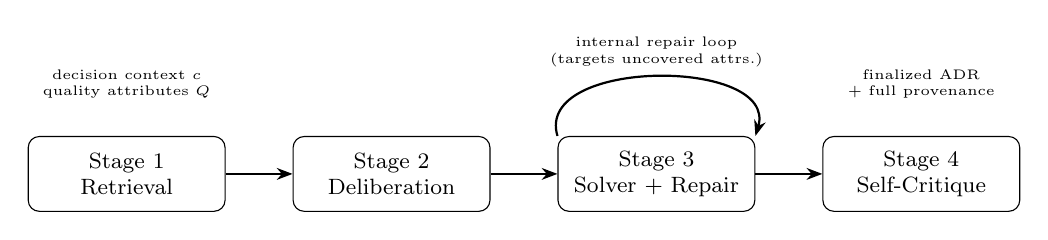
\begin{tikzpicture}[
  stage/.style={draw, rounded corners, minimum width=2.5cm, minimum height=0.95cm, align=center, font=\footnotesize},
  arr/.style={-{Stealth[length=2mm]}, thick},
  node distance=0.85cm
]
\node[stage] (retrieval) {Stage 1\\Retrieval};
\node[stage, right=of retrieval] (delib) {Stage 2\\Deliberation};
\node[stage, right=of delib] (solver) {Stage 3\\Solver + Repair};
\node[stage, right=of solver] (critique) {Stage 4\\Self-Critique};

\draw[arr] (retrieval) -- (delib);
\draw[arr] (delib) -- (solver);
\draw[arr] (solver) -- (critique);

\draw[arr] (solver.north west) .. controls +(-0.3,1.0) and +(0.3,1.0) .. (solver.north east)
  node[midway, above, font=\tiny, align=center] {internal repair loop\\(targets uncovered attrs.)};

\node[above=0.35cm of retrieval, font=\tiny, align=center] {decision context $c$\\quality attributes $Q$};
\node[above=0.35cm of critique, font=\tiny, align=center] {finalized ADR\\+ full provenance};
\end{tikzpicture}
\caption{The CADENCE pipeline. Each stage consumes the previous stage's output; Stage~3's repair loop is internal to Stage~3 --- it never re-enters Stage~2's multi-agent deliberation --- and issues a standalone repair call driven by the solver's uncovered-attribute signal (with the unsatisfiable core reported only as a supplementary diagnostic), iterating to a fixed cap before Stage~4 finalizes the decision.\label{fig:pipeline}}
\end{figure}
\FloatBarrier

\begin{figure}[!htbp]
\centering
\adjustbox{max width=\textwidth}{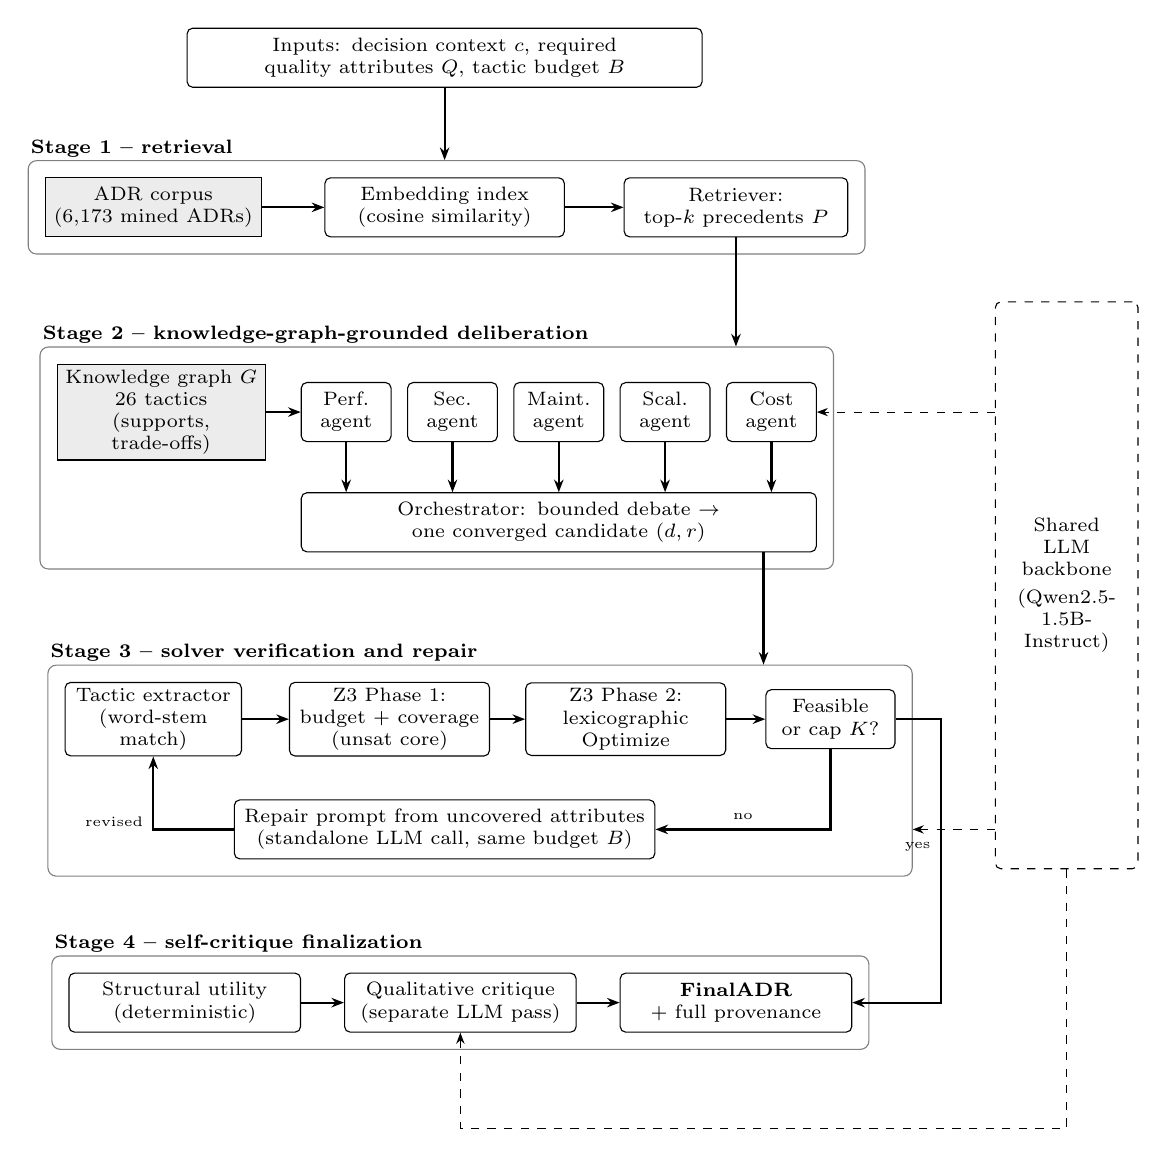
\begin{tikzpicture}[
  font=\scriptsize,
  box/.style={draw, rounded corners=2pt, align=center, minimum height=0.75cm, inner sep=2pt},
  store/.style={draw, align=center, minimum height=0.75cm, inner sep=2pt, fill=gray!15},
  ext/.style={draw, dashed, rounded corners=2pt, align=center, inner sep=3pt},
  layer/.style={draw=gray, rounded corners=3pt, inner xsep=6pt, inner ysep=6pt},
  lbl/.style={font=\scriptsize\bfseries, anchor=south west, inner sep=1pt},
  arr/.style={-{Stealth[length=1.6mm]}, thick},
  darr/.style={-{Stealth[length=1.4mm]}, dashed},
]
% ---- inputs
\node[box, text width=6.4cm] (inp) at (5.2,12.7) {Inputs: decision context $c$, required quality attributes $Q$, tactic budget $B$};

% ---- Stage 1
\node[store, text width=2.6cm] (corpus) at (1.5,10.8) {ADR corpus\\(6{,}173 mined ADRs)};
\node[box, text width=2.9cm] (index) at (5.2,10.8) {Embedding index\\(cosine similarity)};
\node[box, text width=2.7cm] (retr) at (8.9,10.8) {Retriever:\\top-$k$ precedents $P$};
\begin{scope}[on background layer]
\node[layer, fit=(corpus)(index)(retr)] (L1) {};
\end{scope}
\node[lbl] at (L1.north west) {Stage 1 -- retrieval};

% ---- Stage 2
\node[store, text width=2.5cm] (kg) at (1.6,8.2) {Knowledge graph $G$\\26 tactics\\(supports, trade-offs)};
\foreach \x/\n/\t in {3.95/Perf/Perf.,5.3/Sec/Sec.,6.65/Maint/Maint.,8.0/Scal/Scal.,9.35/Cost/Cost}
  \node[box, text width=1.0cm] (ag\n) at (\x,8.2) {\t\\agent};
\node[box, text width=6.4cm] (orch) at (6.65,6.8) {Orchestrator: bounded debate $\rightarrow$ one converged candidate $(d,r)$};
\begin{scope}[on background layer]
\node[layer, fit=(kg)(agPerf)(agCost)(orch)] (L2) {};
\end{scope}
\node[lbl] at (L2.north west) {Stage 2 -- knowledge-graph-grounded deliberation};

% ---- Stage 3
\node[box, text width=2.1cm] (ext) at (1.5,4.3) {Tactic extractor\\(word-stem match)};
\node[box, text width=2.4cm] (z1) at (4.5,4.3) {Z3 Phase 1:\\budget + coverage\\(unsat core)};
\node[box, text width=2.4cm] (z2) at (7.5,4.3) {Z3 Phase 2:\\lexicographic\\Optimize};
\node[box, text width=1.5cm] (dec) at (10.1,4.3) {Feasible\\or cap $K$?};
\node[box, text width=5.2cm] (rep) at (5.2,2.9) {Repair prompt from uncovered attributes\\(standalone LLM call, same budget $B$)};
\begin{scope}[on background layer]
\node[layer, fit=(ext)(z1)(z2)(dec)(rep)] (L3) {};
\end{scope}
\node[lbl] at (L3.north west) {Stage 3 -- solver verification and repair};

% ---- Stage 4
\node[box, text width=2.8cm] (su) at (1.9,0.7) {Structural utility\\(deterministic)};
\node[box, text width=2.8cm] (qc) at (5.4,0.7) {Qualitative critique\\(separate LLM pass)};
\node[box, text width=2.8cm] (fin) at (8.9,0.7) {\textbf{FinalADR}\\+ full provenance};
\begin{scope}[on background layer]
\node[layer, fit=(su)(qc)(fin)] (L4) {};
\end{scope}
\node[lbl] at (L4.north west) {Stage 4 -- self-critique finalization};

% ---- shared LLM backbone
\node[ext, text width=1.6cm, minimum height=7.2cm] (llm) at (13.1,6.0) {Shared\\LLM\\backbone\\[2pt](Qwen2.5-\\1.5B-\\Instruct)};

% ---- main flow
\draw[arr] (inp.south) -- (inp |- L1.north);
\draw[arr] (corpus) -- (index);
\draw[arr] (index) -- (retr);
\draw[arr] (retr.south) -- (retr.south |- L2.north);
\draw[arr] (kg) -- (agPerf);
\foreach \n in {Perf,Sec,Maint,Scal,Cost} \draw[arr] (ag\n.south) -- (ag\n.south |- orch.north);
\draw[arr] ([xshift=2.6cm]orch.south) -- ([xshift=2.6cm]orch.south |- L3.north);
\draw[arr] (ext) -- (z1);
\draw[arr] (z1) -- (z2);
\draw[arr] (z2) -- (dec);
\draw[arr] (dec.south) |- node[pos=0.75,above,font=\tiny]{no} (rep.east);
\draw[arr] (rep.west) -| node[pos=0.55,left,font=\tiny]{revised} (ext.south);
\draw[arr] (dec.east) -- (11.5,4.3) -- node[pos=0.45,left,font=\tiny]{yes} (11.5,0.7) -- (fin.east);
\draw[arr] (su) -- (qc);
\draw[arr] (qc) -- (fin);

% ---- LLM usage (dashed)
\draw[darr] (llm.west |- agCost) -- (agCost.east);
\draw[darr] (llm.west |- rep) -- (L3.east |- rep);
\draw[darr] (llm.south) -- (13.1,-0.9) -- (5.4,-0.9) -- (qc.south);
\end{tikzpicture}
}
\caption{Component architecture of CADENCE. Solid arrows are data flow, dashed arrows are calls to the shared LLM backbone. Stage~1 reads the mined ADR corpus through an embedding index; Stage~2 composes five quality-attribute agents grounded in the tactic knowledge graph~$G$ under one orchestrator; Stage~3 turns the candidate into a Z3 instance and loops through a standalone repair call until the instance is feasible or the repair cap~$K$ is reached; Stage~4 combines a deterministic structural score with a separate LLM critique into the final ADR with full provenance.\label{fig:architecture}}
\end{figure}
\FloatBarrier

\begin{figure}[!htbp]
\centering
\adjustbox{max width=\textwidth}{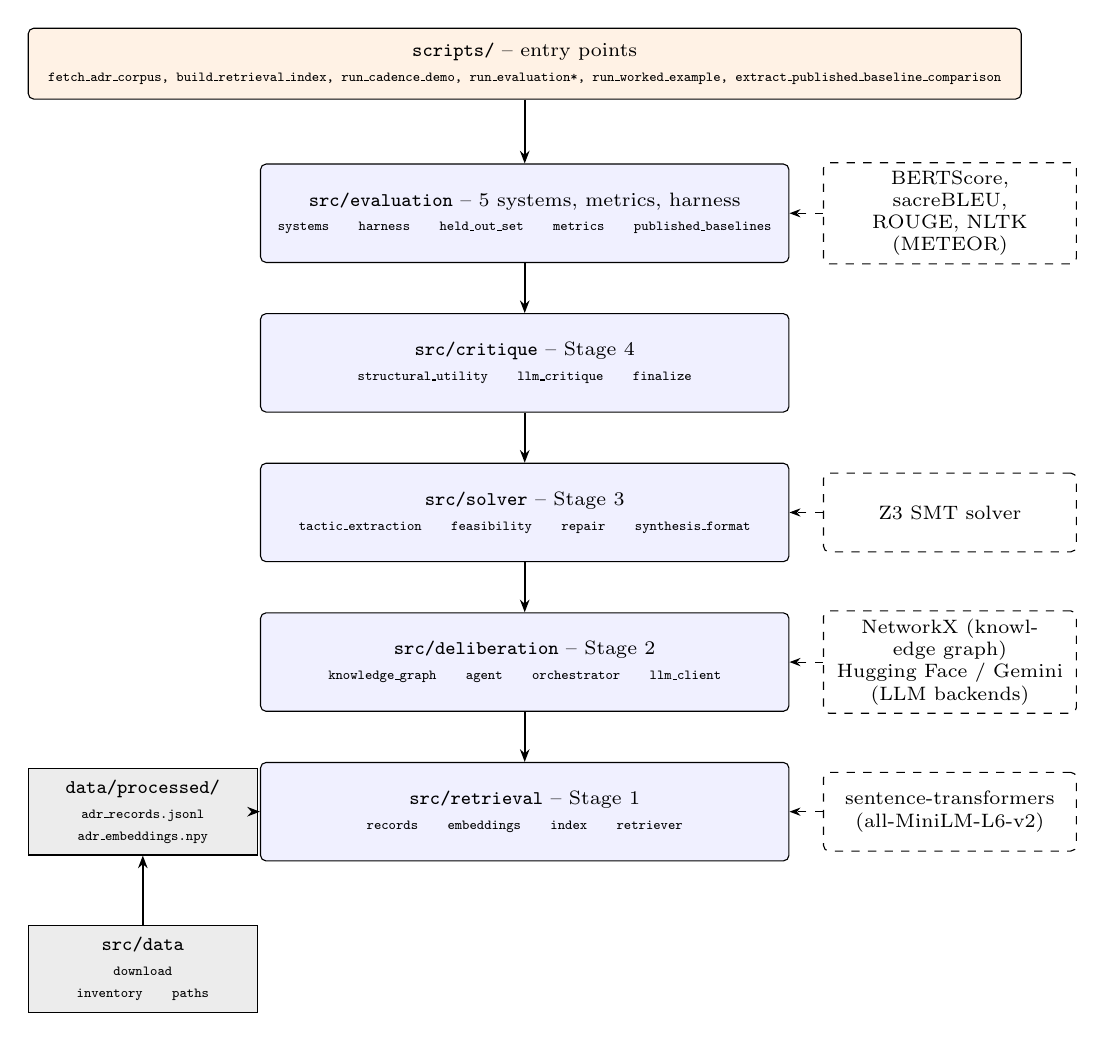
\begin{tikzpicture}[
  font=\scriptsize,
  pkg/.style={draw, rounded corners=2pt, align=center, text width=6.5cm, minimum height=1.25cm, inner sep=3pt, fill=blue!6},
  data/.style={draw, align=center, text width=2.7cm, minimum height=1.1cm, inner sep=3pt, fill=gray!15},
  ext/.style={draw, dashed, rounded corners=2pt, align=center, text width=3.0cm, minimum height=1.0cm, inner sep=3pt},
  top/.style={draw, rounded corners=2pt, align=center, text width=12.4cm, minimum height=0.9cm, inner sep=3pt, fill=orange!10},
  arr/.style={-{Stealth[length=1.6mm]}, thick},
  darr/.style={-{Stealth[length=1.4mm]}, dashed},
]
\node[top] (scripts) at (6.3,10.3) {\textbf{\texttt{scripts/}} -- entry points\\[1pt]{\tiny\ttfamily fetch\_adr\_corpus, build\_retrieval\_index, run\_cadence\_demo, run\_evaluation*, run\_worked\_example, extract\_published\_baseline\_comparison}};

\node[pkg] (ev) at (6.3,8.4) {\textbf{\texttt{src/evaluation}} -- 5 systems, metrics, harness\\[1pt]\modl{systems ~~ harness ~~ held\_out\_set ~~ metrics ~~ published\_baselines}};
\node[pkg] (cr) at (6.3,6.5) {\textbf{\texttt{src/critique}} -- Stage 4\\[1pt]\modl{structural\_utility ~~ llm\_critique ~~ finalize}};
\node[pkg] (so) at (6.3,4.6) {\textbf{\texttt{src/solver}} -- Stage 3\\[1pt]\modl{tactic\_extraction ~~ feasibility ~~ repair ~~ synthesis\_format}};
\node[pkg] (de) at (6.3,2.7) {\textbf{\texttt{src/deliberation}} -- Stage 2\\[1pt]\modl{knowledge\_graph ~~ agent ~~ orchestrator ~~ llm\_client}};
\node[pkg] (re) at (6.3,0.8) {\textbf{\texttt{src/retrieval}} -- Stage 1\\[1pt]\modl{records ~~ embeddings ~~ index ~~ retriever}};

\node[data] (dt) at (1.45,-1.2) {\textbf{\texttt{src/data}}\\[1pt]\modl{download ~~ inventory ~~ paths}};
\node[data] (art) at (1.45,0.8) {\texttt{data/processed/}\\[1pt]\modl{adr\_records.jsonl}\\\modl{adr\_embeddings.npy}};

\node[ext] (e1) at (11.7,0.8) {sentence-transformers\\(all-MiniLM-L6-v2)};
\node[ext] (e2) at (11.7,2.7) {NetworkX (knowledge graph)\\Hugging Face / Gemini\\(LLM backends)};
\node[ext] (e3) at (11.7,4.6) {Z3 SMT solver};
\node[ext] (e4) at (11.7,8.4) {BERTScore, sacreBLEU,\\ROUGE, NLTK (METEOR)};

\draw[arr] (scripts.south -| ev) -- (ev.north);
\draw[arr] (ev) -- (cr);
\draw[arr] (cr) -- (so);
\draw[arr] (so) -- (de);
\draw[arr] (de) -- (re);
\draw[arr] (dt) -- (art);
\draw[arr] (art) -- (re);
\draw[darr] (e1) -- (re);
\draw[darr] (e2) -- (de);
\draw[darr] (e3) -- (so);
\draw[darr] (e4) -- (ev);
\end{tikzpicture}
}
\caption{Software architecture of the released implementation, as a stack of Python packages. Solid arrows are import dependencies between adjacent layers (no package imports from a package above it); dashed arrows are third-party libraries. The retrieval, deliberation, solver and critique packages implement Stages~1--4; the evaluation package re-implements the four baselines and computes the metrics; the data package fetches and inventories the ADR corpus that the retrieval package parses.\label{fig:implementation}}
\end{figure}
\FloatBarrier

\begin{algorithm}[t]
\caption{CADENCE}
\label{alg:cadence}
\begin{algorithmic}[1]
\REQUIRE context $c$, quality attributes $Q$, tactic budget $B$, tactic catalog with graph $G$, max deliberation rounds $R$, max repair iterations $K$
\ENSURE finalized decision with provenance
\STATE $P \gets \textsc{Retrieve}(c)$ \COMMENT{Stage 1: top-$k$ precedents}
\STATE $(d, r) \gets \textsc{Deliberate}(c, P, Q, G, R)$ \COMMENT{Stage 2: bounded multi-agent debate}
\STATE $i \gets 0$; $\mathit{best} \gets \bot$
\LOOP
  \STATE $\mathit{res} \gets \textsc{CheckFeasibility}(d, Q, B, G)$ \COMMENT{Stage 3, Phase 1+2}
  \IF{$\mathit{best} = \bot$ \textbf{or} $|\mathit{res}.\mathit{covered}| > |\mathit{best}.\mathit{res}.\mathit{covered}|$}
    \STATE $\mathit{best} \gets (\mathit{res}, d, r)$ \COMMENT{track highest-coverage attempt seen so far}
  \ENDIF
  \IF{$\mathit{res}.\mathit{feasible}$ \textbf{or} $i = K$}
    \STATE \textbf{break} \COMMENT{degrade gracefully with a caveat if infeasible}
  \ENDIF
  \STATE $(d, r) \gets \textsc{Repair}(d, \mathit{res}.\mathit{uncovered}, B)$ \COMMENT{standalone LLM repair call, targets uncovered attributes}
  \STATE $i \gets i + 1$
\ENDLOOP
\STATE $(\mathit{res}, d, r) \gets \mathit{best}$ \COMMENT{use the best attempt seen, not necessarily the last}
\STATE $u \gets \textsc{StructuralUtility}(\mathit{res}, G)$ \COMMENT{Stage 4, deterministic}
\STATE $q \gets \textsc{QualitativeCritique}(d, r, Q)$ \COMMENT{Stage 4, separate LLM pass}
\RETURN $\textsc{Finalize}(d, r, u, q, \mathit{res}, P)$
\end{algorithmic}
\end{algorithm}

\subsection{Stage 1: Retrieval-Augmented Case-Based Reasoning}

Stage 1 embeds the decision context $c$ with a sentence-embedding model and retrieves the $k$ nearest precedent ADRs, by cosine similarity, from a dense vector index built over the full corpus of $6{,}173$ real, mined ADRs (Section~\ref{sec:evaluation}). Each corpus record is parsed leniently from its source Markdown file --- real-world ADR filenames and internal structure are inconsistent across repositories, so the parser extracts only a title and the full raw body text rather than assuming a fixed section schema. Retrieval returns the top-$k$ precedent records, whose titles are passed into Stage~2 as grounding context; when used inside a held-out evaluation, the query record's own ground-truth ADR is excluded from its own retrieval results to prevent leakage.

\subsection{Stage 2: Knowledge-Graph-Grounded Multi-Agent Deliberation}

Stage 2 instantiates one agent per required quality attribute in $Q$. Each agent is grounded in a knowledge graph $G$ built from a hand-curated catalog of 26 architectural tactics spanning the five quality attributes (5 or 6 per attribute; Table~\ref{tab:tactics} lists the full catalog), where each tactic node has a directed \emph{supports} edge to the quality attribute it primarily serves and directed \emph{trade-off} edges, annotated with a natural-language explanation, to every other attribute it is known to burden --- for instance, \emph{caching} supports \emph{performance} but trades off against \emph{maintainability} via cache-invalidation complexity, and \emph{authentication} supports \emph{security} but trades off against both \emph{performance} (verification latency) and \emph{cost\_operability} (identity-infrastructure upkeep), as Figure~\ref{fig:kg-excerpt} depicts. Given the decision context and Stage~1's retrieved precedents, each agent proposes a candidate decision serving its own attribute using $G$'s \emph{supports} edges, and may critique candidates proposed by other agents; $G$'s \emph{trade-off} edges are consumed downstream by Stage~3's feasibility optimization and Stage~4's utility score, rather than injected into Stage~2's prompts. Deliberation proceeds for a bounded number of rounds ($R$), after which an orchestrator synthesizes the debate into one converged candidate decision and rationale.

\begin{figure}[!htbp]
\centering
\resizebox{\columnwidth}{!}{%
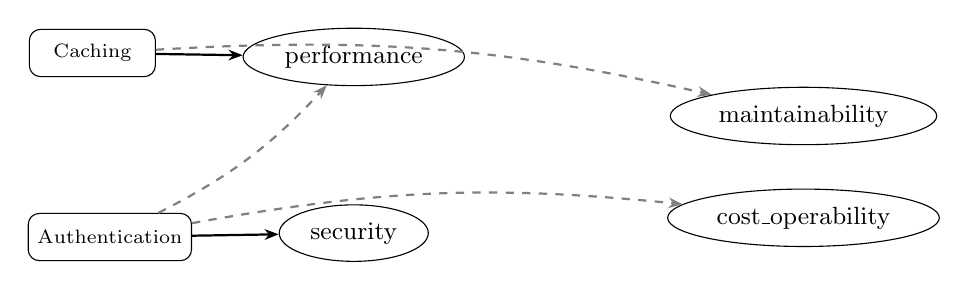
\begin{tikzpicture}[
  qa/.style={draw, ellipse, minimum width=1.55cm, minimum height=0.7cm, align=center, font=\small},
  tac/.style={draw, rounded corners, minimum width=1.6cm, minimum height=0.6cm, align=center, font=\scriptsize},
  supp/.style={-{Stealth[length=1.8mm]}, thick},
  trad/.style={-{Stealth[length=1.8mm]}, dashed, thick, gray},
  node distance=0.55cm and 1.15cm
]
\node[qa] (perf) {performance};
\node[qa, below=1.5cm of perf] (sec) {security};
\node[qa, right=2.6cm of perf, yshift=-0.75cm] (maint) {maintainability};
\node[qa, below=0.55cm of maint] (cost) {cost\_\allowbreak operability};
\node[tac, left=1.1cm of perf, yshift=0.05cm] (caching) {Caching};
\node[tac, left=1.1cm of sec, yshift=-0.05cm] (auth) {Authentication};

\draw[supp] (caching) -- (perf);
\draw[trad] (caching) to[bend left=8] (maint);
\draw[supp] (auth) -- (sec);
\draw[trad] (auth) to[bend right=10] (perf);
\draw[trad] (auth) to[bend left=8] (cost);
\end{tikzpicture}%
}
\caption{Excerpt of knowledge graph $G$: solid arrows are \emph{supports} edges, dashed gray arrows are \emph{trade-off} edges. Only 2 of the catalog's 26 tactics and 4 of its 5 quality attributes are shown for legibility.\label{fig:kg-excerpt}}
\end{figure}
\FloatBarrier

\begin{table}[!htbp]
\caption{The 26-Tactic Catalog Grounding Stage 2's Knowledge Graph $G$. The number in parentheses is the count of \emph{trade-off} edges the tactic carries to other quality attributes (0--2 in this catalog); each tactic's \emph{supports} edge targets the quality attribute in its row.\label{tab:tactics}}
\centering
\footnotesize
\setlength{\tabcolsep}{4pt}
\begin{tabular}{@{}>{\raggedright\arraybackslash}p{0.95in}>{\raggedright\arraybackslash}p{4.25in}@{}}
\toprule
Quality attribute & Tactics (trade-off edges) \\
\midrule
Performance & Caching (1); connection pooling (1); asynchronous processing via message queues (2); data denormalization (1); read-through/write-behind access (1) \\
Security & Authentication (2); fine-grained authorization (1); encryption in transit/at rest (2); rate limiting/throttling (1); least-privilege service boundaries (1); input validation at trust boundaries (1) \\
Maintainability & Modular decomposition by capability (2); versioned API contracts (1); automated regression test suite (1); centralized structured logging (2); dependency injection/IoC (1) \\
Scalability & Horizontal scaling with stateless instances (2); database sharding (2); event-driven architecture (2); auto-scaling infrastructure (1); read replicas (1) \\
Cost/operability & Managed cloud services (2); infrastructure as code (0); multi-tenancy (2); serverless/FaaS deployment (2); circuit breaker for dependencies (1) \\
\bottomrule
\end{tabular}

\vspace{2pt}
\footnotesize \ref{app:catalog} gives each tactic's effect and every trade-off edge with its rationale.
\end{table}
\FloatBarrier

Synthesis is the stage's most format-fragile step: it asks the underlying LLM to emit a two-field response (a one- or two-sentence candidate decision, then a one-paragraph rationale) that Stage~3 can parse deterministically. In practice, real small-model output deviates from any single expected format in ways a fixed parser cannot fully anticipate in advance (Section~\ref{sec:method-robustness}); the orchestrator therefore retries the same synthesis prompt up to three times on a parse failure before surfacing an error, since generation is stochastic and a differently-sampled retry frequently self-corrects a formatting slip that a hand-written regex extension would not have anticipated.

\subsection{Stage 3: Constraint-Solver-Verified Feasibility with Repair Loop}
\label{sec:method-stage3}

Stage 2's converged candidate is free text: a human-readable decision and rationale, not a structured commitment a solver can reason about directly. Stage 3 first extracts which of the 26 catalog tactics the candidate text actually mentions, by word-stem overlap: a tactic counts as mentioned if at least 60\% of the distinct significant words of its name (longer than three letters, excluding stopwords, truncated to four-letter stems) occur among the stems of the candidate text, giving Boolean decision variables $\{t_1, \ldots, t_m\}$, one per mentioned tactic. It then checks feasibility in two phases against the Z3 SMT solver.

\emph{Phase 1 (strict feasibility).} A budget constraint $\sum_i t_i \leq B$ (a caller-specified tactic budget $B$) and, for every required quality attribute $q \in Q$, a coverage constraint $\bigvee_{i \,:\, \mathrm{supports}(t_i) = q} t_i$ (at least one selected tactic must support $q$) are asserted as individually tracked constraints, so that if the instance is unsatisfiable, Z3 returns an \emph{unsatisfiable core}: the constraints jointly responsible for infeasibility. This core is a useful, but not necessarily complete, diagnostic --- Z3's core-extraction semantics can name only one of several symmetric zero-coverage attributes as blocking, omitting others equally unsatisfied --- so Stage~3 does not treat it as authoritative.

\emph{Phase 2 (best-effort optimized selection).} A separate optimization instance re-asserts the budget constraint and searches for the tactic selection that jointly (a) maximizes how many required quality attributes are covered and (b) minimizes the caller-weighted cost of the trade-offs incurred, always returning a concrete selection even when Phase~1 found the instance strictly infeasible. These two objectives are declared to Z3 as separate groups of soft constraints under its lexicographic priority mode, rather than one weighted-sum objective --- a distinction we verified matters empirically. An earlier weighted-sum formulation used a single large constant to bias coverage above trade-off cost, but because trade-off weights are caller-supplied with no upper bound, a selection accumulating enough trade-off weight could mathematically outvote a required attribute's coverage regardless of the bias constant's size (a concrete repro during development: four trade-offs at weight 300 each outweighed a coverage bias of 1000). Lexicographic priority makes coverage strictly dominate trade-off avoidance independent of weight magnitude --- the only encoding safe for caller-supplied weights whose scale cannot be bounded in advance. The resulting split of the required attributes into a covered set and an uncovered set from this phase, not Phase~1's unsat core, is the sound and complete signal of what still needs fixing.

If Phase~1 finds the instance infeasible, Stage~3 constructs a repair prompt naming, for every uncovered attribute, the concrete tactics that would cover it, and asks the LLM to revise the candidate within the same budget. This is re-checked against the solver, iterating up to $K$ times and tracking the best (highest-coverage) attempt seen. If the budget is never satisfiable within the cap, Stage~3 returns the best attempt found with an explicit caveat rather than silently accepting an infeasible decision or discarding an otherwise-reasonable candidate; a transient LLM or parse failure during any repair attempt triggers the next iteration, not an abort.

\subsection{Stage 4: Self-Critique Finalization}
\label{sec:method-stage4}

Stage 4 combines two independently-computed signals into each quality attribute's final utility score. The \emph{structural} component is deterministic: for attribute $q$, it is $1.0$ if $q$ is among the solver-verified decision's covered attributes, minus a fixed penalty of $0.2$ for every incoming trade-off edge from a selected tactic onto $q$ in $G$, floored at $0.0$; it depends only on Stage~3's already-verified output and involves no further LLM call. The \emph{qualitative} component is a single LLM pass scoring every required attribute on a 0--10 scale and flagging any residual weakness, given the full decision, rationale, and attribute list in one call; parsing uses a three-tier matcher --- a strict same-line pattern, a tolerant same-line fallback, and a heading-section fallback for responses that state an attribute as its own heading with the field on a separate, unlabeled line (Section~\ref{sec:method-robustness}) --- so a loose regex cannot lock onto a prose preamble instead of the real scored line, and the call is retried up to three times on a parse failure as Stage~2's synthesis call is. The two components combine as $\mathrm{combined}_q = 0.5 \cdot \mathrm{structural}_q \cdot 10 + 0.5 \cdot \mathrm{qualitative}_q$, and overall decision utility is the mean combined score across all required attributes. The finalized ADR record carries this scoring together with full provenance --- retrieved precedents, the complete per-agent deliberation transcript, which tactics were selected and by which repair iteration, and any solver caveat --- so the decision is auditable end-to-end.

\subsection{Implementation Robustness: Parsing Real, Stochastic LLM Output}
\label{sec:method-robustness}

A structured-output prompt's hand-written happy-path parser reliably breaks against a real, deployed small language model, and our development process surfaced this repeatedly and concretely, not as a theoretical concern. Running the full pipeline end-to-end against Qwen2.5-1.5B-Instruct, the reproducible local backbone used throughout this work, produced six distinct real formatting deviations across Stages~2--4, summarized in Table~\ref{tab:deviations}.

\begin{table}[!htbp]
\caption{Six Real LLM Output-Format Deviations Encountered\label{tab:deviations}}
\centering
\footnotesize
\setlength{\tabcolsep}{3pt}
\begin{tabular}{@{}
  >{\centering\arraybackslash}p{0.15in}
  >{\raggedright\arraybackslash}p{1.55in}
  >{\raggedright\arraybackslash}p{1.65in}
@{}}
\toprule
\# & Deviation & Resolved by \\
\midrule
1 & Extra descriptor word (``Candidate Decision:'' for ``Candidate:'') & Tolerant same-line parser \\
2 & Non-literal ``no weakness'' (``None identified'' for literal ``none'') & Tolerant same-line parser \\
3 & Fraction-style score (``8/10''), this model's \emph{default} 0--10 answer & Tolerant same-line parser \\
4 & Prose preamble a loose regex could lock onto instead of the real line & Tolerant same-line parser \\
5 & Genuine word substitution (``Candidacy:'' for ``Candidate:''), unanticipatable by regex tolerance & Bounded retry (2--3 attempts) \\
6 & Attribute-as-heading structure: attribute on its own heading line, field unlabeled on a later line & Third parser tier (heading-section fallback) \\
\bottomrule
\end{tabular}
\end{table}
\FloatBarrier

The first four are addressable by a sufficiently tolerant same-line parser. The fifth is not, and its discovery motivated this work's general strategy of pairing every structured-output prompt with a bounded retry (two to three attempts) of the identical prompt on a parse failure, rather than special-casing wording variants indefinitely; because generation is stochastic, a differently-sampled retry frequently self-corrects a slip the parser did not anticipate, and Stages~2, 3, and 4 all apply this pattern. The sixth, discovered later during the scaled evaluation run (e.g.\ \texttt{**Performance**} followed, several lines later, by \texttt{**Score:** 9/10} with no attribute name on that line), shows retry's limit: it exhausted all three attempts because it was not a stochastic one-off but a genuinely different \emph{structure} no same-line pattern, however tolerant, could match --- fixing it required a third parser tier (Section~\ref{sec:method-stage4}) that locates an attribute's heading and searches only the bounded section up to the next heading for an unlabeled field. We report this as a methodological finding in its own right: any system asking an LLM for structured intermediate output a downstream deterministic component must consume should validate its parser against real, repeated model output before trusting it unattended, treat bounded retry as the general-purpose fix for wording variation, and expect that a genuinely new structural format will eventually require a genuinely new parser tier --- discoverable only by actually running the real pipeline.

\subsection{Worked Example}
\label{sec:worked-example}

To make the four stages concrete, this section walks through one real, complete run of the pipeline reported as produced by the implementation --- illustrative, not an evaluation data point; this paper's quantitative claims come from Section~\ref{sec:evaluation}'s held-out runs, not this example.

Given a context describing a 10x read-traffic surge on an order-processing service, with requirements to keep p99 latency low, stay operable by a small team, and avoid new security risk, \textbf{Stage 1} retrieves three real precedents on message brokering, server architecture, and JWT inter-service authentication. \textbf{Stage 2} runs two rounds across the five agents: the \emph{performance} agent proposes a message queue to decouple reads from the application server; the \emph{security} agent independently argues for JWT authentication, encryption, and rate limiting; the \emph{cost\_operability} agent's round-2 critique flags a real cross-attribute tension, that the message broker's added network overhead ``could affect real-time interactions.'' The orchestrator synthesizes these into one converged candidate, from which Stage~3 extracts a tactic selection.

\textbf{Stage 3} extracts three catalog tactics --- \emph{asynchronous processing via message queues}, \emph{event-driven architecture}, and \emph{serverless/FaaS deployment} --- covering \emph{performance}, \emph{scalability}, and \emph{cost\_operability}, but not \emph{maintainability} or \emph{security}. This example runs at $B=4$, which, as Section~\ref{sec:evaluation} establishes, cannot cover all five attributes under a catalog where each tactic supports exactly one --- unlike the scaled run's $B=5$ condition, it is not a test of achievable-budget feasibility. It nonetheless illustrates the repair loop's mechanics: one tactic slot remained within budget, but the candidate's text never named a fourth, security- or maintainability-covering tactic for the extractor to find. Both repair attempts fail to close the gap, and Stage~3 returns the best-effort selection with an explicit caveat naming the covered and unaddressed attributes.

\textbf{Stage 4} finalizes the decision --- a microservices architecture using a message queue, an event-sourcing database, and serverless functions --- and scores it per attribute (Table~\ref{tab:worked-example}; Figure~\ref{fig:example-architecture} draws the resulting architecture), flagging a concrete weakness for each (e.g., for \emph{security}: serverless functions carry function-timeout limits and reduced control over the execution environment). The two uncovered attributes' structural components are correctly $0.0$, dragging their combined scores down even where the qualitative pass alone would have scored the prose favorably --- exactly the blending Section~\ref{sec:method-stage4} argues for.

\begin{table}[!htbp]
\caption{Worked Example (Illustrative, $B=4$, Not an Evaluation Data Point): Per-Attribute Utility Scores (Overall: 6.6/10)\label{tab:worked-example}}
\centering
\footnotesize
\begin{adjustbox}{max width=\textwidth}
\begin{tabular}{@{}lccc@{}}
\toprule
Quality Attribute & Structural & Qualitative & Combined \\
\midrule
Performance       & 0.8 & 8.0 & 8.0 \\
Security          & 0.0 & 9.0 & 4.5 \\
Maintainability   & 0.0 & 7.0 & 3.5 \\
Scalability       & 1.0 & 8.0 & 9.0 \\
Cost/Operability  & 1.0 & 6.0 & 8.0 \\
\bottomrule
\end{tabular}
\end{adjustbox}
\end{table}
\FloatBarrier

\begin{figure}[!htbp]
\centering
\adjustbox{max width=\textwidth}{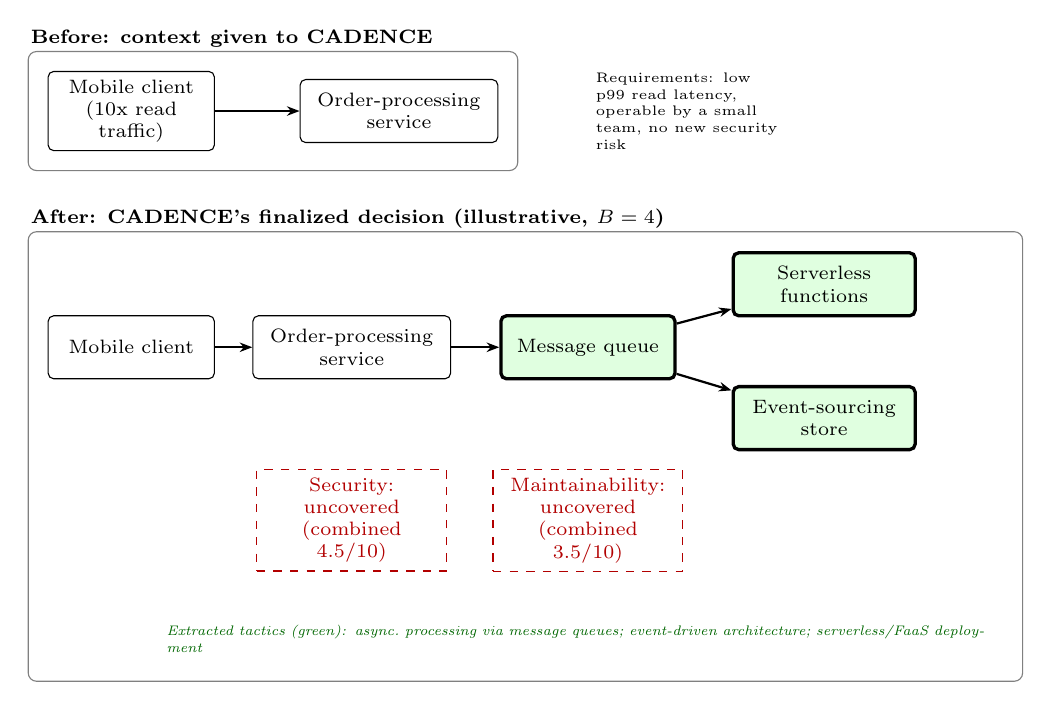
\begin{tikzpicture}[
  font=\scriptsize,
  comp/.style={draw, rounded corners=2pt, align=center, minimum height=0.8cm, inner sep=3pt},
  new/.style={draw, rounded corners=2pt, align=center, minimum height=0.8cm, inner sep=3pt, fill=green!12, very thick},
  gap/.style={draw, dashed, red!70!black, align=center, minimum height=0.8cm, inner sep=3pt, text=red!70!black},
  panel/.style={draw=gray, rounded corners=3pt, inner sep=7pt},
  lbl/.style={font=\scriptsize\bfseries, anchor=south west, inner sep=1pt},
  arr/.style={-{Stealth[length=1.6mm]}, thick},
  tac/.style={font=\tiny\itshape, align=center, text=green!40!black},
]
% ---- before
\node[comp, text width=1.9cm] (mc0) at (1.2,5.2) {Mobile client\\(10x read traffic)};
\node[comp, text width=2.3cm] (os0) at (4.6,5.2) {Order-processing\\service};
\draw[arr] (mc0) -- (os0);
\begin{scope}[on background layer]
\node[panel, fit=(mc0)(os0)] (P0) {};
\end{scope}
\node[lbl] at (P0.north west) {Before: context given to CADENCE};
\node[font=\tiny, align=left, text width=2.4cm] at (8.3,5.2) {Requirements: low p99 read latency, operable by a small team, no new security risk};

% ---- after
\node[comp, text width=1.9cm] (mc) at (1.2,2.2) {Mobile client};
\node[comp, text width=2.3cm] (os) at (4.0,2.2) {Order-processing\\service};
\node[new, text width=2.0cm] (mq) at (7.0,2.2) {Message queue};
\node[new, text width=2.1cm] (fn) at (10.0,3.0) {Serverless\\functions};
\node[new, text width=2.1cm] (es) at (10.0,1.3) {Event-sourcing\\store};
\draw[arr] (mc) -- (os);
\draw[arr] (os) -- (mq);
\draw[arr] (mq) -- (fn);
\draw[arr] (mq) -- (es);
\node[gap, text width=2.2cm] (g1) at (4.0,0.0) {Security: uncovered\\(combined 4.5/10)};
\node[gap, text width=2.2cm] (g2) at (7.0,0.0) {Maintainability: uncovered\\(combined 3.5/10)};
\node[font=\tiny\itshape, text width=10.5cm, align=left, text=green!40!black] (leg) at (6.9,-1.5) {Extracted tactics (green): async.\ processing via message queues; event-driven architecture; serverless/FaaS deployment};
\begin{scope}[on background layer]
\node[panel, fit=(mc)(os)(mq)(fn)(es)(g1)(g2)(leg)] (P1) {};
\end{scope}
\node[lbl] at (P1.north west) {After: CADENCE's finalized decision (illustrative, $B=4$)};
\end{tikzpicture}
}
\caption{The worked example as an architecture. Top: the context given to CADENCE. Bottom: the components named in the finalized decision (green: tactics the extractor found) and the two quality attributes the decision leaves uncovered (red, with their combined utility scores from Table~\ref{tab:worked-example}). The topology is schematic: the run reports which components were selected, not how they are wired.\label{fig:example-architecture}}
\end{figure}
\FloatBarrier

\section{Evaluation}
\label{sec:evaluation}

\subsection{Study Design}
\label{sec:eval-design}

\paragraph{Corpus and task} We evaluate against the ``Context Matters'' replication package~\citep{contextmatters-zenodo} (Zenodo, DOI:~10.5281/zenodo.18370195), which is derived from the same mining study that provides Stage~1's retrieval corpus~\citep{buchgeher2023adr}. The package catalogs 954 repository folders, each with an extraction-confidence status: 750 \textit{Verified}, 96 \textit{Doubt (name sequence)}, 40 \textit{Repo Inaccessible}, 33 \textit{Doubt (no repo dir)}, 30 \textit{Doubt (missing file)} and 5 \textit{Doubt (file contents)}. After parsing, the 882 folders with at least one accessible Markdown file yield 6{,}173 ADR files, with a median of 4, a mean of 7.00 and a maximum of 129 per repository. Held-out items are drawn only from \textit{Verified} folders, so that the quality of the ground truth is not itself a confound. We follow the corpus's own task formulation, ``ADR generation from titles'': each query is a record's title, and the record's full body is the ground truth. A query record is always excluded from its own retrieval results.

\paragraph{Sample} We draw $N=30$ held-out records (seed 44) uniformly from the \textit{Verified} records with at least 300 characters of body text. The six records used in two earlier $N=3$ runs during development (seeds 42 and 43) are excluded, so the sample is disjoint from every item we inspected while building the system. All 30 items completed end to end, with no parse or critique failures.

\paragraph{Configuration} The LLM backbone for every system and every stage is Qwen2.5-1.5B-Instruct, run locally through Hugging Face Transformers on one NVIDIA T4 GPU. Decoding is sampled at temperature 0.7 with at most 400 new tokens per call. Retrieval returns $k=3$ precedents. Deliberation runs $R=2$ rounds (proposals, then one critique round) with the five quality-attribute agents of Section~\ref{sec:method}. The repair loop has $K=2$ attempts. All five attributes are required, with equal weights. We test two tactic budgets. $B=5$ is the smallest feasible budget: each tactic supports exactly one attribute, so five attributes need at least five tactics. $B=7$ adds two tactics of slack, which tests whether the budget, rather than the candidate's content, limits feasibility. One item took about 5 minutes end to end, and the run took 2.5 hours.

\paragraph{Paired design} For each item, Stages~1 and~2 run once, and every downstream system consumes that same output. \sysMA{} is the deliberation's candidate. Stage~3 is then run on that candidate once per budget, giving \sysNC{}, and Stage~4 runs on the resulting verified decision, giving \sysFull{}. Adjacent systems therefore differ in exactly one stage on identical input, and the two budget conditions share one deliberation. The two earlier development runs did not have this property, because each system re-ran Stages~1--3 independently; Section~\ref{sec:eval-earlier} explains why this matters.

\subsection{Systems Compared}

The systems form an ablation ladder in which each step adds one stage:
\begin{itemize}[leftmargin=*,itemsep=1pt,topsep=2pt,parsep=0pt]
\item \sysZS{}: a single LLM call given only the decision context, the baseline style of \citet{dhar2024llm}.
\item \sysRO{}: the context plus the titles of Stage~1's top-$k$ precedents, the retrieval-augmented style of \citet{contextmatters2026}.
\item \sysMA{}: Stages~1--2. This is the deliberation's converged candidate and rationale, comparable to multi-agent ADR generation such as MAAD~\citep{zhang2025maad} but with quality-attribute advocates instead of functional roles.
\item \sysNC{}: Stages~1--3. The candidate after solver verification and, where it is infeasible, repair.
\item \sysFull{}: Stages~1--4. Stage~4 scores the verified decision; it does not rewrite it (Section~\ref{sec:method-stage4}). The decision and rationale text of \sysFull{} is therefore identical to that of \sysNC{}. What Stage~4 adds is the per-attribute utility scores and the residual weaknesses. To let the text metrics see that addition, we also score \sysFull{}+Cons., in which the residual weaknesses are appended as a ``Consequences'' section. This is the section in which an ADR conventionally records the negative effects of a decision~\citep{tyree2005}.
\end{itemize}

\subsection{Measures and Analysis}

\paragraph{Agreement with the recorded decision} We report the four metrics used in the LLM-for-ADR studies we compare against~\citep{dhar2024llm,contextmatters2026}: BERTScore F1 (roberta-large, no baseline rescaling), sentence-level BLEU (sacreBLEU, 0--100), ROUGE-1 F1 (with stemming) and METEOR. Each output is compared with the human-authored body of the held-out ADR. These metrics measure agreement with one recorded decision, not decision quality. Their limits for software-engineering text are well documented~\citep{roy2021,evtikhiev2023,haque2022}, and RQ4 examines them directly.

\paragraph{Feasibility} For Stage~3 we report the constraint-satisfaction rate (the share of items for which the decision covers all required attributes within $B$) and the number of attributes covered. We also report the coverage of the deliberation's candidate \emph{before} repair, by applying Stage~3's deterministic tactic extraction to it. This separates what deliberation contributes from what repair contributes.

\paragraph{Statistics} Every comparison is paired by item. For each adjacent pair on the ladder we report the mean paired difference with a 95\% percentile bootstrap interval (10{,}000 resamples), the count of items on which each system wins, and a two-sided Wilcoxon signed-rank test. Within each metric, we adjust the $p$-values for the eleven comparisons with Holm's method. A difference is called significant when the Holm-adjusted $p<0.05$.

\subsection{RQ1: What Does Each Stage Contribute?}
\label{sec:rq1}

\begin{table}[!htbp]
\caption{Mean agreement with the held-out human-authored ADRs ($N=30$, paired), with 95\% bootstrap intervals, and median output length in words (reference ADRs: median 163, mean 289).\label{tab:rq1-means}}
\centering
\begin{adjustbox}{max width=\textwidth}
\begin{tabular}{@{}lccccr@{}}
\toprule
System & BERTScore F1 & BLEU & ROUGE-1 F1 & METEOR & Words \\
\midrule
\sysZS{}  & 0.813 {\tiny[0.809, 0.818]} & 1.90 {\tiny[1.41, 2.47]} & 0.255 {\tiny[0.232, 0.275]} & 0.223 {\tiny[0.202, 0.243]} & 301 \\
\sysRO{}  & 0.817 {\tiny[0.813, 0.821]} & 1.90 {\tiny[1.41, 2.48]} & 0.265 {\tiny[0.246, 0.283]} & 0.227 {\tiny[0.206, 0.246]} & 300 \\
\sysMA{}  & 0.804 {\tiny[0.799, 0.810]} & 0.56 {\tiny[0.34, 0.81]} & 0.144 {\tiny[0.122, 0.168]} & 0.084 {\tiny[0.068, 0.103]} & 90 \\
\midrule
\sysNC{}, $B=5$  & 0.799 {\tiny[0.794, 0.803]} & 0.58 {\tiny[0.40, 0.79]} & 0.148 {\tiny[0.132, 0.163]} & 0.093 {\tiny[0.077, 0.109]} & 120 \\
\sysFull{}, $B=5$  & 0.799 {\tiny[0.794, 0.803]} & 0.58 {\tiny[0.40, 0.79]} & 0.148 {\tiny[0.132, 0.163]} & 0.093 {\tiny[0.077, 0.109]} & 120 \\
\sysFull{}+Cons., $B=5$  & 0.802 {\tiny[0.798, 0.806]} & 0.66 {\tiny[0.50, 0.84]} & 0.178 {\tiny[0.161, 0.193]} & 0.134 {\tiny[0.120, 0.148]} & 233 \\
\midrule
\sysNC{}, $B=7$  & 0.802 {\tiny[0.797, 0.807]} & 0.58 {\tiny[0.37, 0.83]} & 0.147 {\tiny[0.128, 0.168]} & 0.089 {\tiny[0.074, 0.105]} & 107 \\
\sysFull{}, $B=7$  & 0.802 {\tiny[0.797, 0.808]} & 0.58 {\tiny[0.37, 0.83]} & 0.147 {\tiny[0.128, 0.168]} & 0.089 {\tiny[0.074, 0.105]} & 107 \\
\sysFull{}+Cons., $B=7$  & 0.805 {\tiny[0.800, 0.810]} & 0.66 {\tiny[0.48, 0.85]} & 0.175 {\tiny[0.157, 0.191]} & 0.124 {\tiny[0.110, 0.139]} & 209 \\
\bottomrule
\end{tabular}
\end{adjustbox}
\end{table}

\begin{table}[!htbp]
\caption{Paired differences along the ablation ladder ($N=30$): mean difference (later minus earlier system), with wins/losses of the later system in parentheses; ties are omitted. $^{*}$: Holm-adjusted Wilcoxon $p<0.05$ within the metric.\label{tab:rq1-paired}}
\centering
\begin{adjustbox}{max width=\textwidth}
\begin{tabular}{@{}lcccc@{}}
\toprule
Step (stage added) & BERTScore F1 & BLEU & ROUGE-1 F1 & METEOR \\
\midrule
\sysZS{} $\to$ \sysRO{} (retrieval) & +0.004$^{*}$ (22/8) & +0.01 (15/15) & +0.010 (21/9) & +0.004 (15/15) \\
\sysRO{} $\to$ \sysMA{} (deliberation) & $-$0.013$^{*}$ (3/27) & $-$1.35$^{*}$ (4/26) & $-$0.120$^{*}$ (3/27) & $-$0.142$^{*}$ (0/30) \\
\sysMA{} $\to$ \sysNC{}, $B=5$ (solver, repair) & $-$0.006$^{*}$ (0/17) & +0.02 (14/3) & +0.003 (12/5) & +0.008 (14/3) \\
\sysMA{} $\to$ \sysNC{}, $B=7$ (solver, repair) & $-$0.002 (5/9) & +0.02 (9/4) & +0.002 (9/4) & +0.005 (10/3) \\
\sysNC{} $\to$ \sysFull{}, both $B$ (critique) & 0 (0/0) & 0 (0/0) & 0 (0/0) & 0 (0/0) \\
\sysNC{} $\to$ \sysFull{}+Cons., $B=5$ & +0.003$^{*}$ (22/8) & +0.07 (18/12) & +0.031$^{*}$ (21/9) & +0.041$^{*}$ (27/3) \\
\sysNC{} $\to$ \sysFull{}+Cons., $B=7$ & +0.003$^{*}$ (26/4) & +0.08 (18/12) & +0.028$^{*}$ (22/8) & +0.035$^{*}$ (29/1) \\
\midrule
\sysZS{} $\to$ \sysFull{}, $B=5$ (whole pipeline) & $-$0.015$^{*}$ (3/27) & $-$1.31$^{*}$ (7/23) & $-$0.107$^{*}$ (1/29) & $-$0.130$^{*}$ (0/30) \\
\bottomrule
\end{tabular}
\end{adjustbox}
\end{table}

\begin{figure}[!htbp]
\centering
\adjustbox{max width=\textwidth}{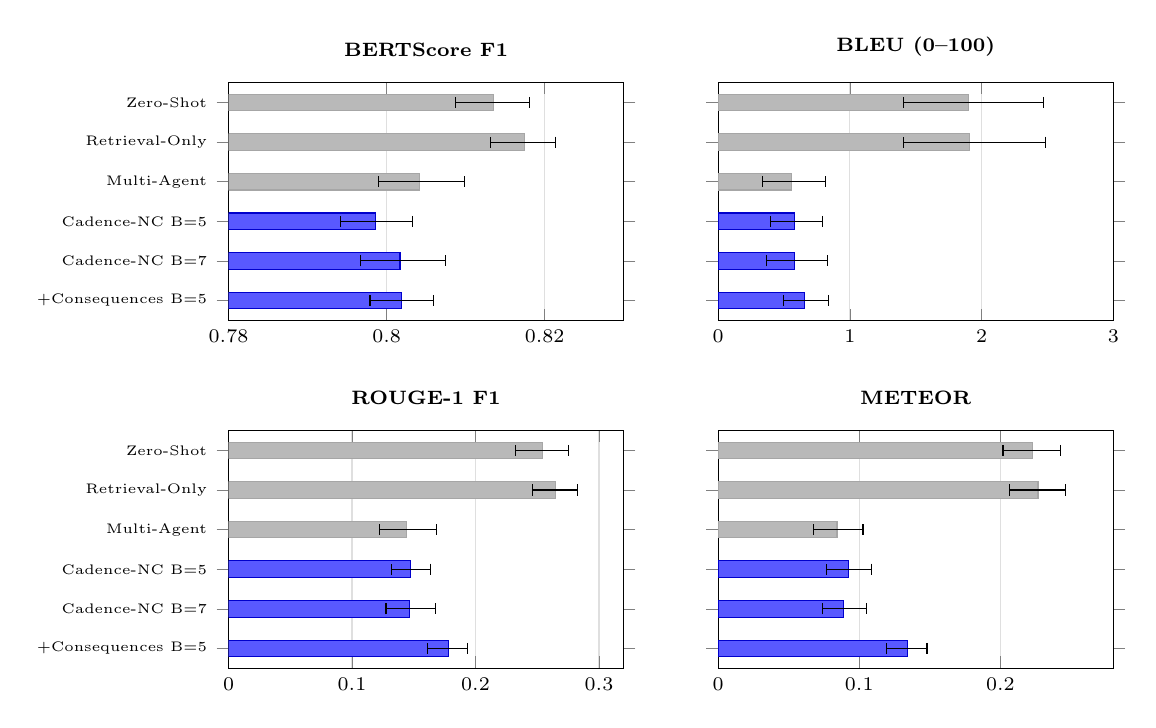
\begin{tikzpicture}
\pgfplotsset{every axis/.append style={
  width=6.6cm, height=4.6cm, xbar, bar width=6pt, enlarge y limits=0.1,
  symbolic y coords={Zero-Shot,Retrieval-Only,Multi-Agent,Cadence-NC B=5,Cadence-NC B=7,+Consequences B=5},
  ytick={Zero-Shot,Retrieval-Only,Multi-Agent,Cadence-NC B=5,Cadence-NC B=7,+Consequences B=5}, y dir=reverse, font=\scriptsize, y tick label style={font=\tiny},
  title style={font=\scriptsize\bfseries}, xmajorgrids, grid style={gray!25}, x tick label style={/pgf/number format/fixed}}}
\begin{groupplot}[group style={group size=2 by 2, horizontal sep=1.2cm, vertical sep=1.4cm, yticklabels at=edge left}]
\nextgroupplot[title={BERTScore F1}, xmin=0.78, xmax=0.83, xtick={0.78,0.80,0.82}]
\addplot[fill=gray!55, draw=gray!70, bar shift=0pt, error bars/.cd, x dir=both, x explicit, error bar style={black}] coordinates {(0.8135,Zero-Shot) += (0.0046,0) -= (0.0048,0) (0.8174,Retrieval-Only) += (0.0040,0) -= (0.0042,0) (0.8042,Multi-Agent) += (0.0057,0) -= (0.0052,0)};
\addplot[fill=blue!65, draw=blue!80!black, bar shift=0pt, error bars/.cd, x dir=both, x explicit, error bar style={black}] coordinates {(0.7986,Cadence-NC B=5) += (0.0047,0) -= (0.0044,0) (0.8017,Cadence-NC B=7) += (0.0058,0) -= (0.0050,0) (0.8019,+Consequences B=5) += (0.0040,0) -= (0.0040,0)};
\nextgroupplot[title={BLEU (0--100)}, xmin=0, xmax=3, xtick={0,1,2,3}]
\addplot[fill=gray!55, draw=gray!70, bar shift=0pt, error bars/.cd, x dir=both, x explicit, error bar style={black}] coordinates {(1.8973,Zero-Shot) += (0.5702,0) -= (0.4901,0) (1.9048,Retrieval-Only) += (0.5775,0) -= (0.4972,0) (0.5596,Multi-Agent) += (0.2552,0) -= (0.2229,0)};
\addplot[fill=blue!65, draw=blue!80!black, bar shift=0pt, error bars/.cd, x dir=both, x explicit, error bar style={black}] coordinates {(0.5826,Cadence-NC B=5) += (0.2069,0) -= (0.1826,0) (0.5780,Cadence-NC B=7) += (0.2515,0) -= (0.2130,0) (0.6559,+Consequences B=5) += (0.1835,0) -= (0.1593,0)};
\nextgroupplot[title={ROUGE-1 F1}, xmin=0, xmax=0.32, xtick={0,0.1,0.2,0.3}]
\addplot[fill=gray!55, draw=gray!70, bar shift=0pt, error bars/.cd, x dir=both, x explicit, error bar style={black}] coordinates {(0.2546,Zero-Shot) += (0.0209,0) -= (0.0224,0) (0.2645,Retrieval-Only) += (0.0184,0) -= (0.0187,0) (0.1443,Multi-Agent) += (0.0238,0) -= (0.0224,0)};
\addplot[fill=blue!65, draw=blue!80!black, bar shift=0pt, error bars/.cd, x dir=both, x explicit, error bar style={black}] coordinates {(0.1476,Cadence-NC B=5) += (0.0158,0) -= (0.0157,0) (0.1467,Cadence-NC B=7) += (0.0210,0) -= (0.0192,0) (0.1781,+Consequences B=5) += (0.0153,0) -= (0.0167,0)};
\nextgroupplot[title={METEOR}, xmin=0, xmax=0.28, xtick={0,0.1,0.2}]
\addplot[fill=gray!55, draw=gray!70, bar shift=0pt, error bars/.cd, x dir=both, x explicit, error bar style={black}] coordinates {(0.2228,Zero-Shot) += (0.0199,0) -= (0.0210,0) (0.2266,Retrieval-Only) += (0.0196,0) -= (0.0203,0) (0.0842,Multi-Agent) += (0.0184,0) -= (0.0165,0)};
\addplot[fill=blue!65, draw=blue!80!black, bar shift=0pt, error bars/.cd, x dir=both, x explicit, error bar style={black}] coordinates {(0.0925,Cadence-NC B=5) += (0.0162,0) -= (0.0159,0) (0.0890,Cadence-NC B=7) += (0.0159,0) -= (0.0148,0) (0.1340,+Consequences B=5) += (0.0140,0) -= (0.0144,0)};
\end{groupplot}
\end{tikzpicture}
}
\caption{Mean agreement with the held-out ADRs and 95\% bootstrap intervals ($N=30$). Grey: single-pass and deliberation-only systems; blue: systems that include Stage~3. \sysFull{} is omitted because its text equals \sysNC{}'s. The BERTScore axis starts at 0.78.\label{fig:results}}
\end{figure}
\FloatBarrier

Tables~\ref{tab:rq1-means} and~\ref{tab:rq1-paired} and Figure~\ref{fig:results} report the results.

\emph{Retrieval} gives a small but consistent gain in BERTScore (+0.004, 22 of 30 items, significant). It does not change the surface metrics significantly.

\emph{Deliberation} is the largest effect in the study, and it is negative on every metric. Against \sysRO{}, \sysMA{} loses on BERTScore in 27 of 30 items and on METEOR in all 30. Its output is also much shorter (median 90 words against 300). This is by design: the synthesis prompt asks for a one-line decision and a short rationale that Stage~3 can parse. RQ4 tests how much of the loss is due to length alone.

\emph{Solver verification and repair} leave the decision text unchanged on the 13 items (at $B=5$) where repair did not improve coverage, because the loop then returns the original candidate. On the 17 changed items, repaired text is slightly closer to the reference on the surface metrics (14 of 17 items on BLEU and METEOR), but no such difference is significant. BERTScore drops slightly but significantly at $B=5$ ($-0.006$). The solver stage is thus roughly neutral for agreement with the recorded decision. Its value has to be judged on feasibility (RQ2).

\emph{Critique} does not change the text at all, so its difference on every metric is exactly zero. Rendering Stage~4's residual weaknesses as a Consequences section improves BERTScore, ROUGE-1 and METEOR significantly at both budgets; METEOR improves on 27 and 29 of 30 items. The section roughly doubles the output length, however, so this is partly a length effect (RQ4). It does indicate that what the critique identifies overlaps with what architects actually wrote down.

Taken as a whole, the full pipeline agrees less with the recorded ADRs than one zero-shot call does, on all four metrics.

\subsection{RQ2: Does Solver Verification Make Decisions Feasible?}
\label{sec:rq2}

\begin{figure}[!htbp]
\centering
\adjustbox{max width=\textwidth}{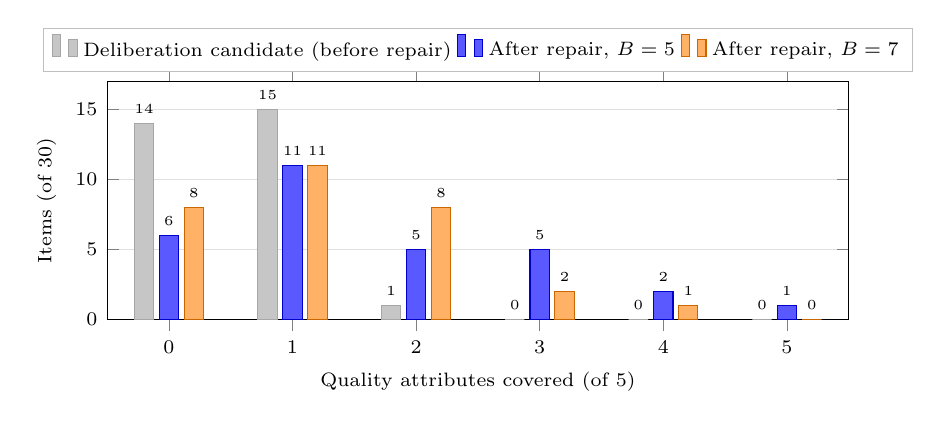
\begin{tikzpicture}
\begin{axis}[
  width=11cm, height=4.6cm, ybar, bar width=7pt, ymin=0, ymax=17,
  xlabel={Quality attributes covered (of 5)}, ylabel={Items (of 30)},
  xtick={0,1,2,3,4,5}, font=\scriptsize, ymajorgrids, grid style={gray!25},
  legend style={font=\scriptsize, at={(0.5,1.04)}, anchor=south, legend columns=3, draw=gray!50},
  nodes near coords, every node near coord/.append style={font=\tiny},
]
\addplot[fill=gray!45, draw=gray!70] coordinates {(0,14) (1,15) (2,1) (3,0) (4,0) (5,0)};
\addplot[fill=blue!65, draw=blue!80!black] coordinates {(0,6) (1,11) (2,5) (3,5) (4,2) (5,1)};
\addplot[fill=orange!60, draw=orange!80!black] coordinates {(0,8) (1,11) (2,8) (3,2) (4,1) (5,0)};
\legend{{Deliberation candidate (before repair)},{After repair, $B=5$},{After repair, $B=7$}}
\end{axis}
\end{tikzpicture}
}
\caption{Number of required quality attributes (of five) covered by the decision's tactic commitments, per item ($N=30$): the deliberation's candidate before repair, and the best candidate after up to $K=2$ repairs at each budget. Feasibility requires all five.\label{fig:coverage}}
\end{figure}

\begin{table}[!htbp]
\caption{Solver outcomes ($N=30$). Coverage is the number of required quality attributes (of five) covered within the budget.\label{tab:rq2}}
\centering
\begin{adjustbox}{max width=\textwidth}
\begin{tabular}{@{}lccc@{}}
\toprule
 & Before repair & After repair, $B=5$ & After repair, $B=7$ \\
\midrule
Feasible items & 0/30 & 1/30 & 0/30 \\
Mean attributes covered & 0.57 & 1.63 & 1.23 \\
Items with zero coverage & 14 & 6 & 8 \\
Items whose coverage repair improved & --- & 17 & 13 \\
Mean repair attempts used & --- & 2.00 & 2.00 \\
\bottomrule
\end{tabular}
\end{adjustbox}
\end{table}
\FloatBarrier

Table~\ref{tab:rq2} and Figure~\ref{fig:coverage} report the solver's view of the same 30 decisions.

\emph{Deliberated decisions rarely commit to catalog tactics, and when they do, the tactics cluster on one attribute.} Before repair, 14 of 30 candidates name no tactic from the catalog, and 15 cover a single attribute. The mean is 0.57 of five. This holds even though every agent's prompt lists the tactics for its attribute (\ref{app:p-agent}). The converged decision often keeps only the decision's subject; one candidate reads in full ``Akka Persistence''. When a candidate does name several tactics, they tend to come from one group. ``Use asynchronous processing via message queues, caching, connection pooling, and data denormalization'' names four tactics, all of which support performance. The advocates for the other four attributes argued during the rounds, but their concerns did not survive into the synthesized decision.

\emph{Repair helps, but not enough.} Repair raises mean coverage to 1.63 attributes at $B=5$ and improves 17 of 30 items. It reaches full coverage once: on one item, the second repair produced a decision naming five tactics, one per attribute. Every other item exhausted both repair attempts.

\emph{Slack does not help.} At $B=7$, no item is feasible, and coverage is lower than at $B=5$ (1.23; 12 items are better at $B=5$, 7 at $B=7$). The candidates and solver encoding are identical across budgets, so the difference comes entirely from the stochastic repair calls. The number of tactics is not what binds. Repaired candidates often name more tactics than either budget allows, up to 18 in one case. What binds is \emph{diversity}: the named tactics support too few distinct attributes. A larger budget cannot fix a decision that is silent on security.

This is the answer to RQ2 for this backbone: formal verification works as a \emph{detector}. On all 30 items it correctly reports that the decision leaves required attributes unaddressed, and it names which ones. Bounded repair through the same small model does not turn that detection into feasible decisions. Section~\ref{sec:discussion} discusses what this implies for the design.

\subsection{RQ3: Comparison with Published Frontier-Model Generations}
\label{sec:published-comparison}

%%RQ3%%

\subsection{RQ4: How Well Do Reference-Based Metrics Capture the Difference?}
\label{sec:rq4}

\begin{table}[!htbp]
\caption{Length-controlled comparison ($N=30$). Each baseline's output is truncated, per item, to the word count of \sysNC{} ($B=5$) on that item. Differences are \sysNC{} minus the truncated baseline; wins/losses of \sysNC{} in parentheses; $^{*}$: Holm-adjusted $p<0.05$.\label{tab:rq4}}
\centering
\begin{adjustbox}{max width=\textwidth}
\begin{tabular}{@{}lcccc@{}}
\toprule
 & BERTScore F1 & BLEU & ROUGE-1 F1 & METEOR \\
\midrule
\sysZS{}, full length & 0.813 & 1.90 & 0.255 & 0.223 \\
\sysZS{}, truncated  & 0.812 & 1.80 & 0.234 & 0.177 \\
\sysRO{}, truncated  & 0.814 & 1.81 & 0.246 & 0.178 \\
\sysNC{}, $B=5$ & 0.799 & 0.58 & 0.148 & 0.093 \\
\midrule
\sysNC{} vs.\ \sysZS{}, truncated & $-$0.013$^{*}$ (2/28) & $-$1.22$^{*}$ (1/29) & $-$0.087$^{*}$ (0/30) & $-$0.085$^{*}$ (0/30) \\
\sysNC{} vs.\ \sysRO{}, truncated & $-$0.015$^{*}$ (3/27) & $-$1.23$^{*}$ (0/30) & $-$0.098$^{*}$ (0/30) & $-$0.086$^{*}$ (0/30) \\
\bottomrule
\end{tabular}
\end{adjustbox}
\end{table}
\FloatBarrier

CADENCE's outputs are 2.5--3 times shorter than the baselines' (Table~\ref{tab:rq1-means}). Length does track the surface metrics: across all systems and items, the ratio of output length to reference length correlates with ROUGE-1 (Spearman $\rho=0.26$, $p<10^{-4}$, 270 system--item pairs). To isolate length, Table~\ref{tab:rq4} truncates each baseline's output to \sysNC{}'s length on the same item.

Truncation closes only part of the gap. Against \sysZS{}, length accounts for about a fifth of the ROUGE-1 gap (from 0.107 to 0.087) and a third of the METEOR gap (from 0.130 to 0.085). At equal length, the baselines still win on every metric and on nearly every item, BERTScore included. In the earlier, $N=3$ version of this work, we read the gap between surface metrics and BERTScore as an artifact of output length. That reading does not survive the length control.

The remaining gap reflects what the text says. An ADR as architects write it has a context, a decision, and consequences, in project-specific vocabulary. The single-pass baselines imitate that form. CADENCE's output is a decision statement plus a rationale phrased in quality-attribute and tactic terms, and the reference ADRs rarely use that vocabulary. A metric based on similarity to the reference cannot distinguish ``different from what this team wrote'' from ``worse'', and so cannot credit the stages whose purpose is to change the decision's content: making trade-offs explicit, and checking coverage. Measuring those stages calls for instruments other than reference agreement, such as expert assessment of whether the decision addresses the stated quality concerns.

\subsection{Earlier Development Runs}
\label{sec:eval-earlier}

During development we ran two smaller evaluations, each with $N=3$ items (seeds 42 and 43). Unlike the paired run, each system there re-ran Stages~1--3 independently. In the second of those runs, \sysFull{} scored above \sysNC{} on 7 of 8 budget--metric comparisons, and we reported this as a positive signal for self-critique. The paired design shows that this was not a critique effect. Stage~4 never changes the decision text, so the difference came entirely from two independent samples of the same stochastic deliberation. This is why the paired design is necessary for ablating stochastic multi-stage pipelines. The other patterns from those runs do reproduce at $N=30$: zero feasible items at $B=5$, deliberation-based systems far below the single-pass baselines on ROUGE-1 and METEOR, and a narrower gap on BERTScore.

\section{Discussion}
\label{sec:discussion}

\subsection{Verification as a Detector: Where the Pipeline Loses Quality-Attribute Commitments}

The central result is a mismatch between two stages. The quality-attribute advocates do raise their concerns, and Stage~3 checks precisely whether the decision addresses those concerns. Between the two, however, Stage~2's synthesis compresses the debate into a one-line decision, and the concerns of four of the five advocates rarely survive the compression (Section~\ref{sec:rq2}). Stage~3 then reports this correctly on 29 of 30 items. Repairing the text afterwards, with the same 1.5B model, recovers coverage only partially.

This locates the problem at the interface between language and formal model, not in the solver. The architecture-optimization literature assumes a design space that experts specify in a formal model~\citep{aleti2013,martens2010,koziolek2011peropteryx}. CADENCE instead extracts the design space from generated text, and the extraction is only as rich as the text. Three design changes follow from the data, and each can be tested with the same paired protocol:
\begin{enumerate}[leftmargin=*]
\item \emph{Make the decision structured.} Instead of matching tactic names in free text, the synthesis step could emit an explicit commitment per attribute, for example ``security: least-privilege service boundaries''. Constrained decoding could keep it inside the catalog. Coverage then becomes a property of the output format, and the solver's job reduces to checking budget and trade-offs.
\item \emph{Repair at the deliberation, not after it.} The uncovered attributes reported by Stage~3 could be returned to the corresponding advocate agents for another round, rather than to a stand-alone repair prompt that sees only the synthesized decision.
\item \emph{Let the solver choose and the LLM explain.} With a given catalog and the stated requirements, the solver can select a feasible, minimal-trade-off tactic set on its own. Deliberation would then argue about which feasible set fits the context and write the rationale. This reverses the roles, and moves CADENCE closer to search-based design-space exploration with an LLM front end.
\end{enumerate}
Each change also benefits from a richer, empirically grounded tactic model. The 26-tactic catalog, with one supported attribute per tactic, could be checked and extended against mined tactic--quality-attribute knowledge~\citep{bi2021} and tactic--pattern interaction models~\citep{harrison2010,marquez2023}.

\subsection{Implications for Practitioners}

For teams that already use LLMs to draft ADRs, the results support two practical steps. First, a draft that reads well does not necessarily address the team's quality concerns. In our sample, the deliberated drafts left on average more than four of five required attributes without a named tactic. Second, the check that exposes this is cheap. Stage~3's tactic extraction is deterministic, the solver instance is tiny, and neither needs a large model. A coverage report that names which required attributes a draft leaves unaddressed is a useful review aid even when no automatic repair follows. Stage~4's residual weaknesses, rendered as a Consequences section, are a second inexpensive addition. They make the draft agree significantly more with what architects recorded (Section~\ref{sec:rq1}). The final decision remains a human responsibility. The influence factors that dominate real decisions, such as team expertise, organizational constraints and existing commitments~\citep{weinreich2015}, are not in the title-only task context CADENCE receives here.

\subsection{Implications for Research on LLM-Assisted Architecture}

Two methodological lessons apply beyond CADENCE.

The first concerns \emph{reference-based metrics}. They measure imitation of one recorded decision. The length-controlled analysis (Section~\ref{sec:rq4}) shows that a system can trail on every such metric for reasons other than output length, simply because it writes in a different vocabulary than the recorded ADR. This matches findings for code summarization and code generation~\citep{roy2021,evtikhiev2023,haque2022}. Small metric differences between LLM-for-ADR systems should therefore not be read as differences in decision quality. Stages that are meant to change content, such as trade-off reasoning and coverage checking, need instruments that measure that content: expert ratings against the stated quality concerns, or task-based evaluation with practitioners. LLM judges are a tempting substitute. Their agreement with human raters in software-engineering tasks varies, however, and same-family judging adds self-preference bias~\citep{wang2025judge,he2026judge}. Stage~4's critique is itself an LLM judge of this kind, which is why we do not report its scores as evidence of quality.

The second concerns \emph{ablating stochastic pipelines}. When each system variant re-samples the shared upstream stages, differences between variants mix stage effects with sampling noise. On three items this noise was large enough to look like a consistent critique effect (Section~\ref{sec:eval-earlier}). Sharing upstream outputs across variants, and testing paired differences, is a simple remedy, and we recommend it for any multi-stage LLM evaluation.

\subsection{Threats to Validity}

\paragraph{Construct validity} Agreement with one human-authored ADR is a proxy for decision quality. A decision can differ from the recorded one and still be sound, and the recorded one may itself be poor. We address this by reporting feasibility separately and by analyzing the metrics directly (RQ4), but we collected no expert judgments. Stage~3's coverage measure depends on matching tactic names in text. A decision that addresses an attribute in words not in the catalog is counted as not covering it. Some of the low coverage may be due to this, although the agents' prompts list the exact tactic names.

\paragraph{Internal validity} All systems share one backbone, decoding configuration and prompt set (\ref{app:prompts}). Results may depend on these choices, in particular on the 1.5B backbone, whose limited instruction following plausibly contributes to the compression problem. Generation is sampled, and each item ran once. The paired design removes sampling variance from the comparisons between Stage~2 and later stages, but not from the comparisons among the first three systems, which use independent calls.

\paragraph{External validity} The items come from open-source projects that publish ADRs, and the task gives only the ADR's title as context. Decisions in industrial settings, with richer context and different documentation practices, may behave differently. The five quality attributes and 26 tactics are a deliberately small subset of published catalogs~\citep{marquez2023}.

\paragraph{Conclusion validity} With $N=30$, small effects such as retrieval's +0.004 BERTScore are detectable only because pairing removes between-item variance. We adjust for multiple comparisons within each metric. The feasibility result (1 of 30 at $B=5$) is clear-cut. A rate close to zero is consistent with these data, but a moderate rate under a stronger backbone is not ruled out.

\subsection{Engineering Lessons for Solver-Verified LLM Pipelines}

Two implementation findings generalize. First, the lexicographic encoding in Stage~3 (Section~\ref{sec:method-stage3}) is required whenever callers can set weights on a secondary objective: under a weighted sum, a large enough trade-off weight silently overrides a requirement the caller believed was hard. Second, when a deterministic component consumes structured LLM output, a tolerant parser alone does not converge. Models produce novel format deviations that no regular expression anticipates. A bounded retry of the same prompt (Section~\ref{sec:method-robustness}) avoids these deviations by exploiting sampling variability, without enumerating them in advance.

\section{Conclusion}
\label{sec:conclusion}

We presented CADENCE, an approach to LLM-assisted architectural decision-making that combines precedent retrieval from mined ADRs, deliberation among quality-attribute advocates grounded in a tactic knowledge graph, verification of the decision's tactic commitments with an SMT solver, and a scored critique. Its aim is to join two lines of software architecture research that have developed separately: LLM-based ADR generation, which produces fluent decisions without checking them, and tactic-based and search-based architecture design, which checks decisions but needs a formal model specified by hand.

A paired evaluation on 30 held-out ADRs from open-source projects gives a clear picture for a small local backbone. Retrieval helps slightly. Multi-agent deliberation lowers agreement with the recorded decisions, by more than output length explains. Solver verification is a reliable detector: it reports, correctly, that 29 of 30 deliberated decisions leave required quality attributes without a committed tactic. Repair improves coverage but makes only one decision feasible, and budget slack does not help, because the binding constraint is the diversity of the committed tactics, not their number. Stage~4 does not change the decision text. Its residual weaknesses, rendered as consequences, do bring the text closer to what architects wrote. The paired design also corrected an earlier small-sample finding that had credited the critique stage with gains caused by sampling noise.

Future work follows from these findings: structured, catalog-constrained decision output; feedback of uncovered attributes to the advocate agents; solver-first selection of tactic sets; an empirically grounded tactic model; stronger backbones; and evaluation by architects of whether decisions address their quality concerns, rather than by agreement with a single recorded text.

\section*{Data and Code Availability}
This paper is self-contained: the tactic catalog and every prompt are given in \ref{app:catalog} and~\ref{app:prompts}, and all reported numbers appear in the tables. The implementation, the processed corpus, the evaluation scripts, the per-item outputs and solver diagnostics of the paired evaluation, and the statistical analysis are available at:

\begin{center}
\footnotesize\url{https://github.com/vinhqdang/Large-Language-Models-in-Service-Oriented-Ecosystems-Design}
\end{center}

The underlying ADR corpus is the public ``Context Matters'' replication package~\citep{contextmatters-zenodo}.

\section*{Acknowledgments}
The author thanks the maintainers of the ``Context Matters'' ADR replication package for making a real, richly annotated ADR corpus publicly available, without which this work's retrieval stage and evaluation would not have been possible.


\appendix
\section{Tactic catalog}
\label{app:catalog}

Table~\ref{tab:catalog-full} lists all 26 tactics of the knowledge graph $G$. Each tactic has one \emph{supports} edge, to the quality attribute of its group, and the \emph{trade-off} edges shown in the last column, each with the reason it burdens the named attribute. Trade-off edges are the only cross-attribute relations in $G$; Stage~3 minimizes their weighted cost and Stage~4 deducts a penalty for each one that lands on an attribute. The catalog is hand-curated in original wording from widely documented architectural concepts, not mined from the ADR corpus.

{\footnotesize
\setlength{\tabcolsep}{3pt}
\begin{longtable}{@{}>{\raggedright\arraybackslash}p{1.35in}>{\raggedright\arraybackslash}p{1.65in}>{\raggedright\arraybackslash}p{2.22in}@{}}
\caption{Full tactic catalog: effect and trade-off edges (target attribute and reason) for each of the 26 tactics.\label{tab:catalog-full}}\\
\toprule
Tactic & Effect & Trade-off edges \\
\midrule
\endfirsthead
\toprule
Tactic & Effect & Trade-off edges \\
\midrule
\endhead
\bottomrule
\endfoot
\multicolumn{3}{@{}l}{\textbf{Performance}} \\
\midrule
Caching & Store frequently-accessed results to avoid recomputation or repeated I/O. & \emph{maintainability}: cache invalidation and staleness become an ongoing concern \\
Connection pooling & Reuse expensive connections (DB, network) instead of opening one per request. & \emph{maintainability}: pool sizing and lifecycle tuning adds operational complexity \\
Asynchronous processing via message queues & Decouple slow work from the request path via a queue and background workers. & \emph{maintainability}: harder to trace an end-to-end request across queue boundaries; \emph{security}: the queue and its consumers become additional attack surface \\
Data denormalization & Duplicate data to avoid expensive joins or cross-service calls at read time. & \emph{maintainability}: duplicated data must be kept consistent across writers \\
Read-through/write-behind data access & Batch or defer writes and prefetch reads to reduce per-operation latency. & \emph{maintainability}: failure windows can lose or reorder deferred writes \\
\midrule
\multicolumn{3}{@{}l}{\textbf{Security}} \\
\midrule
Authentication & Verify the identity of a caller before granting access. & \emph{performance}: adds per-request latency for credential verification; \emph{cost/operability}: requires identity infrastructure to run and maintain \\
Fine-grained authorization / access control & Restrict operations to callers with the specific permissions they need. & \emph{maintainability}: permission policies must be kept in sync with the system's evolution \\
Encryption in transit and at rest & Protect data from interception or unauthorized disk-level access. & \emph{performance}: adds CPU overhead for encrypt/decrypt operations; \emph{cost/operability}: key management and rotation is an ongoing operational task \\
Rate limiting / throttling & Cap how much load a single caller can place on the system. & \emph{performance}: adds bookkeeping overhead to every request, including legitimate ones \\
Least-privilege service boundaries & Give each service only the access it strictly needs, isolating blast radius. & \emph{maintainability}: more, narrower services means more boundaries to coordinate changes across \\
Input validation at trust boundaries & Reject malformed or malicious input as early as possible. & \emph{performance}: adds validation overhead on every incoming request \\
\midrule
\multicolumn{3}{@{}l}{\textbf{Maintainability}} \\
\midrule
Modular decomposition by business capability & Split the system along business boundaries so each module changes independently. & \emph{performance}: cross-module calls add latency that a single module wouldn't have; \emph{cost/operability}: more independently deployable units means more to operate \\
Versioned, well-defined API contracts & Make module/service boundaries explicit and evolve them without breaking consumers. & \emph{cost/operability}: contract review and versioning tooling adds process overhead \\
Automated regression test suite & Catch behavioral regressions automatically before they reach production. & \emph{cost/operability}: CI compute time and suite upkeep is a recurring cost \\
Centralized structured logging and observability & Make system behavior inspectable across components for debugging and audits. & \emph{cost/operability}: log storage and processing infrastructure has an ongoing cost; \emph{security}: logs can leak sensitive data if not deliberately scrubbed \\
Dependency injection / inversion of control & Decouple components from concrete implementations of their dependencies. & \emph{performance}: the extra indirection has a small but nonzero runtime cost \\
\midrule
\multicolumn{3}{@{}l}{\textbf{Scalability}} \\
\midrule
Horizontal scaling with stateless instances & Add more identical instances behind a load balancer instead of growing one instance. & \emph{cost/operability}: more running instances means more infrastructure to pay for and operate; \emph{maintainability}: session/request state must be externalized, not held in-process \\
Database sharding & Partition data across multiple database instances by a shard key. & \emph{maintainability}: cross-shard queries and rebalancing become genuinely hard problems; \emph{cost/operability}: operating multiple database instances multiplies operational surface \\
Event-driven architecture & Components communicate via events rather than direct synchronous calls. & \emph{maintainability}: reasoning about system state requires tracing asynchronous event flows; \emph{security}: each event channel is an additional integration point to secure \\
Auto-scaling infrastructure & Automatically add or remove capacity in response to observed load. & \emph{performance}: newly-started instances suffer cold-start latency during scale-up \\
Read replicas & Serve read traffic from replicated copies of the primary data store. & \emph{maintainability}: callers must tolerate and reason about replication lag \\
\midrule
\multicolumn{3}{@{}l}{\textbf{Cost/operability}} \\
\midrule
Managed cloud services over self-hosted infrastructure & Use a vendor-operated service instead of running and patching the equivalent yourself. & \emph{security}: trust and blast radius now partly depend on the vendor's shared-responsibility model; \emph{maintainability}: the system becomes coupled to that vendor's specific service semantics \\
Infrastructure as code & Define infrastructure declaratively so environments are reproducible and cheap to recreate. & none \\
Multi-tenancy & Share infrastructure across multiple customers/tenants instead of provisioning per-tenant. & \emph{security}: a boundary failure between tenants has a much larger blast radius; \emph{performance}: a noisy tenant can degrade performance for others sharing the same resources \\
Serverless / function-as-a-service deployment & Pay only for actual invocation time instead of provisioning always-on capacity. & \emph{performance}: cold starts add latency to infrequently-invoked functions; \emph{maintainability}: execution model constraints (timeouts, statelessness) shape how code must be written \\
Circuit breaker for downstream dependencies & Stop calling a failing dependency instead of paying for retries against it. & \emph{maintainability}: failure-handling logic and fallback paths add real code complexity \\
\end{longtable}
}

\section{Prompt templates}
\label{app:prompts}

All prompts used by the pipeline and baselines are reproduced below; angle brackets mark values filled in at run time. Agents (Stage~2) receive the system prompt in Section~\ref{app:p-agent} with every call; all other calls have no system prompt. $\langle a\rangle$ is a quality attribute, $\langle c\rangle$ the decision context, and precedent lines are the titles of the $k$ retrieved ADRs.

\subsection{Stage 2: quality-attribute agent}\label{app:p-agent}
\begin{lstlisting}
[system]
You are the <a> advocate in an architectural decision-making deliberation. Argue for the decision that best serves <a>, while acknowledging real trade-offs.
Tactics you can draw on for <a>: <names of the tactics supporting <a>, comma-separated>

[round 1, propose]
Decision context:
<c>

Precedent decisions from similar past projects:
- <title of precedent 1>
- ...

Propose and justify a position from the <a> perspective for this decision.

[rounds 2..R, critique]
Current candidate decision:
<all agents' latest positions, one per line>

Other advocates' positions this round:
- [<attribute>] <position>
- ...

From the <a> perspective, critique or refine this candidate, citing specific trade-offs where relevant.
\end{lstlisting}

\subsection{Stage 2: synthesis}
\begin{lstlisting}
Decision context:
<c>

Full deliberation transcript:
[<attribute> r<round>] <position>
...

Synthesize the deliberation into a final decision. Respond in exactly this format:
CANDIDATE: <one or two sentence decision>
RATIONALE: <one paragraph rationale>
\end{lstlisting}

\subsection{Stage 3: repair}
\begin{lstlisting}
The following architectural decision candidate cannot be verified as feasible:
<current candidate>

Constraint: the decision may commit to at most <B> distinct architectural tactics (an operability budget).
Required quality attributes that must each be addressed by at least one tactic: <Q, comma-separated>.
The best attempt so far leaves these quality attributes unaddressed: <uncovered attributes> (at least <unsat-core attributes> are known to conflict with the budget).

Tactics you could name explicitly to address each unaddressed attribute:
- <uncovered attribute>: <names of the tactics supporting it>
- ...

Revise the decision to fit within the tactic budget while covering as many of the required quality attributes as possible -- naming specific tactics from the lists above by name where you use them -- consolidating around fewer, higher-impact tactics where needed. Respond in exactly this format:
CANDIDATE: <one or two sentence decision>
RATIONALE: <one paragraph rationale>
\end{lstlisting}

\subsection{Stage 4: qualitative critique}
\begin{lstlisting}
Decision: <decision>
Rationale: <rationale>

Critique this architectural decision from each quality attribute perspective below. Score each 0 (fails this attribute) to 10 (exemplary), and name one specific residual weakness if any exist (or 'none'). Respond in exactly this format, one block per attribute:
<ATTRIBUTE>_SCORE: <0-10>
<ATTRIBUTE>_WEAKNESS: <specific weakness, or 'none'>
... (one block for each required attribute)
\end{lstlisting}

\subsection{Baselines}
\begin{lstlisting}
[Zero-Shot]
Decision context:
<c>

Write an architectural decision record addressing this context.

[Retrieval-Only]
Decision context:
<c>

Precedent decisions from similar past projects:
- <title of precedent 1>
- ...

Write an architectural decision record addressing this context, informed by the precedents above.
\end{lstlisting}

\bibliographystyle{elsarticle-harv}
\bibliography{cadence_ist}

\end{document}
